% Options for packages loaded elsewhere
\PassOptionsToPackage{unicode}{hyperref}
\PassOptionsToPackage{hyphens}{url}
\PassOptionsToPackage{dvipsnames,svgnames,x11names}{xcolor}
%
\documentclass[
  12,
  letterpaper,
  DIV=11,
  numbers=noendperiod]{scrartcl}

\usepackage{amsmath,amssymb}
\usepackage{lmodern}
\usepackage{iftex}
\ifPDFTeX
  \usepackage[T1]{fontenc}
  \usepackage[utf8]{inputenc}
  \usepackage{textcomp} % provide euro and other symbols
\else % if luatex or xetex
  \usepackage{unicode-math}
  \defaultfontfeatures{Scale=MatchLowercase}
  \defaultfontfeatures[\rmfamily]{Ligatures=TeX,Scale=1}
\fi
% Use upquote if available, for straight quotes in verbatim environments
\IfFileExists{upquote.sty}{\usepackage{upquote}}{}
\IfFileExists{microtype.sty}{% use microtype if available
  \usepackage[]{microtype}
  \UseMicrotypeSet[protrusion]{basicmath} % disable protrusion for tt fonts
}{}
\makeatletter
\@ifundefined{KOMAClassName}{% if non-KOMA class
  \IfFileExists{parskip.sty}{%
    \usepackage{parskip}
  }{% else
    \setlength{\parindent}{0pt}
    \setlength{\parskip}{6pt plus 2pt minus 1pt}}
}{% if KOMA class
  \KOMAoptions{parskip=half}}
\makeatother
\usepackage{xcolor}
\setlength{\emergencystretch}{3em} % prevent overfull lines
\setcounter{secnumdepth}{5}
% Make \paragraph and \subparagraph free-standing
\ifx\paragraph\undefined\else
  \let\oldparagraph\paragraph
  \renewcommand{\paragraph}[1]{\oldparagraph{#1}\mbox{}}
\fi
\ifx\subparagraph\undefined\else
  \let\oldsubparagraph\subparagraph
  \renewcommand{\subparagraph}[1]{\oldsubparagraph{#1}\mbox{}}
\fi


\providecommand{\tightlist}{%
  \setlength{\itemsep}{0pt}\setlength{\parskip}{0pt}}\usepackage{longtable,booktabs,array}
\usepackage{calc} % for calculating minipage widths
% Correct order of tables after \paragraph or \subparagraph
\usepackage{etoolbox}
\makeatletter
\patchcmd\longtable{\par}{\if@noskipsec\mbox{}\fi\par}{}{}
\makeatother
% Allow footnotes in longtable head/foot
\IfFileExists{footnotehyper.sty}{\usepackage{footnotehyper}}{\usepackage{footnote}}
\makesavenoteenv{longtable}
\usepackage{graphicx}
\makeatletter
\def\maxwidth{\ifdim\Gin@nat@width>\linewidth\linewidth\else\Gin@nat@width\fi}
\def\maxheight{\ifdim\Gin@nat@height>\textheight\textheight\else\Gin@nat@height\fi}
\makeatother
% Scale images if necessary, so that they will not overflow the page
% margins by default, and it is still possible to overwrite the defaults
% using explicit options in \includegraphics[width, height, ...]{}
\setkeys{Gin}{width=\maxwidth,height=\maxheight,keepaspectratio}
% Set default figure placement to htbp
\makeatletter
\def\fps@figure{htbp}
\makeatother
\newlength{\cslhangindent}
\setlength{\cslhangindent}{1.5em}
\newlength{\csllabelwidth}
\setlength{\csllabelwidth}{3em}
\newlength{\cslentryspacingunit} % times entry-spacing
\setlength{\cslentryspacingunit}{\parskip}
\newenvironment{CSLReferences}[2] % #1 hanging-ident, #2 entry spacing
 {% don't indent paragraphs
  \setlength{\parindent}{0pt}
  % turn on hanging indent if param 1 is 1
  \ifodd #1
  \let\oldpar\par
  \def\par{\hangindent=\cslhangindent\oldpar}
  \fi
  % set entry spacing
  \setlength{\parskip}{#2\cslentryspacingunit}
 }%
 {}
\usepackage{calc}
\newcommand{\CSLBlock}[1]{#1\hfill\break}
\newcommand{\CSLLeftMargin}[1]{\parbox[t]{\csllabelwidth}{#1}}
\newcommand{\CSLRightInline}[1]{\parbox[t]{\linewidth - \csllabelwidth}{#1}\break}
\newcommand{\CSLIndent}[1]{\hspace{\cslhangindent}#1}

\KOMAoption{captions}{tableheading}
\usepackage{tikz}
\usepackage{pgfplots}
\pgfplotsset{compat=newest}
\usetikzlibrary{plotmarks}
\usetikzlibrary{arrows.meta}
\usepgfplotslibrary{patchplots}
\usepackage{grffile}
\usepackage{caption}
\usepackage[utf8]{inputenc}
\usepackage[doublespacing]{setspace}
\AtBeginEnvironment{tabular}{\singlespacing}
\usepackage{float}
\usepackage{multirow}
\usepackage{tablefootnote}
\usepackage{pifont}
\usepackage{newunicodechar}
\usepackage{booktabs}
\usepackage{siunitx}
\usepackage{tabularx}
\newunicodechar{✓}{\ding{51}}
\makeatletter
\makeatother
\makeatletter
\makeatother
\makeatletter
\@ifpackageloaded{caption}{}{\usepackage{caption}}
\AtBeginDocument{%
\ifdefined\contentsname
  \renewcommand*\contentsname{Table of contents}
\else
  \newcommand\contentsname{Table of contents}
\fi
\ifdefined\listfigurename
  \renewcommand*\listfigurename{List of Figures}
\else
  \newcommand\listfigurename{List of Figures}
\fi
\ifdefined\listtablename
  \renewcommand*\listtablename{List of Tables}
\else
  \newcommand\listtablename{List of Tables}
\fi
\ifdefined\figurename
  \renewcommand*\figurename{Figure}
\else
  \newcommand\figurename{Figure}
\fi
\ifdefined\tablename
  \renewcommand*\tablename{Table}
\else
  \newcommand\tablename{Table}
\fi
}
\@ifpackageloaded{float}{}{\usepackage{float}}
\floatstyle{ruled}
\@ifundefined{c@chapter}{\newfloat{codelisting}{h}{lop}}{\newfloat{codelisting}{h}{lop}[chapter]}
\floatname{codelisting}{Listing}
\newcommand*\listoflistings{\listof{codelisting}{List of Listings}}
\makeatother
\makeatletter
\@ifpackageloaded{caption}{}{\usepackage{caption}}
\@ifpackageloaded{subcaption}{}{\usepackage{subcaption}}
\makeatother
\makeatletter
\@ifpackageloaded{tcolorbox}{}{\usepackage[many]{tcolorbox}}
\makeatother
\makeatletter
\@ifundefined{shadecolor}{\definecolor{shadecolor}{rgb}{.97, .97, .97}}
\makeatother
\makeatletter
\makeatother
\ifLuaTeX
  \usepackage{selnolig}  % disable illegal ligatures
\fi
\IfFileExists{bookmark.sty}{\usepackage{bookmark}}{\usepackage{hyperref}}
\IfFileExists{xurl.sty}{\usepackage{xurl}}{} % add URL line breaks if available
\urlstyle{same} % disable monospaced font for URLs
\hypersetup{
  pdftitle={Allies as Armaments: Explaining the Specialization of State Military Capabilities},
  pdfauthor={J Andrés Gannon},
  colorlinks=true,
  linkcolor={blue},
  filecolor={Maroon},
  citecolor={Blue},
  urlcolor={Blue},
  pdfcreator={LaTeX via pandoc}}

\title{Allies as Armaments: Explaining the Specialization of State
Military Capabilities\thanks{The author is thankful to many who provided
feedback on earlier and related drafts, including but not limited to
Steven Brooks, Rosella Cappella Zielinski, Jonathan Cavereley, Rex
Douglass, Benjamin O. Fordham, Erik Gartzke, Stacie Goddard, Nadiya
Kostyuk, Kendrick Kuo, David Lake, Brett Ashley Leeds, Erik
Lin-Greenberg, Paul MacDonald, Michaela Mattes, Steven Miller, Sara
Plana, Paul Poast, Abigail Post, Philip Roeder, Sebastian Rosato, Erik
Sand, Thomas Leo Scherer, Kaija Schilde, Todd Sechser, Branislav
Slantchev, Jennifer Spindel, Sanne Verschuren, and many others. This
project could not have happened without help from the many research
assistants helped construct the rDMC dataset on which this article
relies, This project benefited from financial support from the UC San
Diego Center for Peace and Security Studies (cPASS), Harvard Kennedy
School Belfer Center for Science and International Affairs, the Smith
Richardson Foundation, Stanton Nuclear Foundation, the Department of
Defense Minerva Initiative, the Charles Koch Foundation, and the APSA
Centennial Center.}}
\author{J Andrés Gannon}
\date{July 19, 2023}

\begin{document}
\maketitle
\begin{abstract}
\singlespacing \noindent Why do states under-produce some military
capabilities and over-produce others in ways that seem to leave them
vulnerable? This article argues alliances help explain states' decisions
to specialize defense. By reducing the risks of under-producing some
capabilities and creating an incentive to over-produce others, alliances
enable states to achieve the benefits of specialization and
diversification simultaneously. Using granular military capability data,
this paper develops the first systematic measurement of military
specialization and finds states with militarily-capable alliance
partners are more likely to specialize their own militaries. This
finding suggests a new interplay between seemingly opposing strategies
for defense that challenges existing perspectives on internal versus
external balancing. In identifying how alliances shape the composition
of arms, these findings have important implications for current debates
about burden-sharing and motivate future research explaining armament
decisions and the consequences of alliances.
\end{abstract}
\ifdefined\Shaded\renewenvironment{Shaded}{\begin{tcolorbox}[borderline west={3pt}{0pt}{shadecolor}, boxrule=0pt, frame hidden, sharp corners, breakable, interior hidden, enhanced]}{\end{tcolorbox}}\fi

\newpage

\hypertarget{sec-intro}{%
\section{Introduction}\label{sec-intro}}

Despite constitutional restrictions on its military, Japan began
shifting its defense investments in the late 1970's. By 1982, Prime
Minster Suzuki had drawn up plans to overhaul Japan's military by
investing primarily in air defense and light offshore surface ships
designed the counter the concerning increase in Soviet naval forces
(Modly 1985). Although the end of the Cold War marked the end of the
Soviet threat in the Western Pacific, it was soon replaced with Japanese
concerns about Chinese expansion and the island-chain state's
vulnerability to a blockade (Suzuki and Wallace 2018). But over the
following decade, Japan's defense capabilities continued shifting and by
the turn of the century Japan had doubled its air defense and
short-range aerial capabilities but almost completely phased out its
amphibious fleet and coastal ships, despite their clear utility in
countering a potential blockade (Twomey 2000, 185--88; Lind 2004,
107--10). In specializing in air defense while neglecting amphibious and
coastal capabilities, Japan's military portfolio appears to have left it
unnecessarily vulnerable.

This is exemplary of a common phenomenon in international politics.
Conventional wisdom holds that because the primary purpose of a state's
military is to provide security against perceived foreign dangers (Waltz
1979, 102--14), most states should invest in a diversified full-spectrum
force, hedging their bets in an unpredictable international environment
by compensating for the inherent weaknesses of any one set of
capabilities, or prioritize strengthening defenses against the most
salient threats (Biddle 2005, 199--200). However, there are myriad
examples like Japan's of a capable state possessing a seemingly
vulnerable military that specializes by under-producing some
capabilities and over-producing others. The US omitted minesweepers
during President Reagan's 600-ship rebuilding plan despite their low
cost and the fact that 13 of the 15 US ships sunk since World War II
were victims of naval mines -- a decision that caused serious problems
in the late 1980's during the Iran-Iraq Tanker War (Till 2005). Given
its 225 mile coastline, Albania's decision in the early 2000's to
purchase dozens of open-water patrol vessels that could reach Portugal's
coast 1,750 miles away seems a poor fit for their self-defense needs,
especially considering the disintegration of the military and looting of
defense installations just a few years prior left them without any
functioning battle tanks (Hendrickson, Campbell, and Mullikin 2006,
253--54; Polak, Hendrickson, and Garrett 2009). Estonia's sophisticated
cyber capabilities have been frequently lauded, but those sizable
investments have occurred alongside divestment of their entire combat
aircraft fleet, even in the presence of increasingly warranted concern
about Russian aggression and possible invasion (Andžāns and Veebel
2017). Why do some countries have gaps in their militaries that they
could fill, but choose not to, or excesses and redundancies they could
avoid, but maintain?

My central argument is that the extent to which a state specializes its
defense capabilities can, in part, be explained by alliance
participation. Alliances reduce the costs of forgoing some defense
assets and also increase the benefits of over-producing others. By
gaining protection from your allies' armaments, alliances allow states
to simultaneously garner the benefits of a collectively diversified set
of arms while lowering the risk of -- and creating an additional
incentive for -- individually specialized militaries. The result is
variation in the composition of military capabilities across states -
some being comparatively more specialized. Empirically, this paper
examines state-level military specialization and alliance relationships
from 1970 to 2014 and finds that states with more militarily-capable
alliance partners specialize their militaries more than those with weak
or non-existent allies. When it comes to zero-sum resource allocation to
defense, alliances allow states to have their cake and eat it, too,
garnering the benefits of diversification and specialization
simultaneously.

This article makes a number of contributions to the study of
international politics. For one, it develops the first rigorous and
systematic measurement of an important, yet under-studied dimension of
armament decisions: military specialization. Despite a general
acceptance that militaries differ, scholars have been unable to identify
those differences in degree or kind. In doing so, this paper also
introduces a novel theory of specialization within alliances that has
significant implications for our understanding of two foundational
trade-offs in international politics: guns versus butter (R. Powell
1993; Poast 2019b) and external versus internal balancing (Altfeld 1984;
Morrow 1993). Diversifying one's ``guns'' may maximize security under
anarchy, but it produces a higher defense burden that necessitates less
resources available for ``butter''. But by influencing the \emph{types}
of armaments states produce, alliances can minimize that guns versus
butter trade-off through specialization-induced efficiency improvements
(Kinne and Kang 2023)\emph{.} Regarding the second trade-off, although
states can provide for their defense by arming (internal balancing) or
forming alliances (external balancing), a common and influential view
holds there are inherent inefficiencies and risks associated with the
latter (Walt 1985; Oneal 1990). Because self-interested states only
abide by international agreements that involve decisions they would have
made otherwise (Downs, Rocke, and Barsoom 1996, 388--90), attempts to
jointly produce public goods like security through alliances that are
little more than ``temporary marriages of convenience'' (Mearsheimer
1994, 11) are inevitably haunted by incentives to exploit, renege, and
free ride (Olson and Zeckhauser 1966, 3; Snyder 1984). But alliances do
not jointly produce security simply by aggregating defense (Morrow
1991); alliances \emph{reconstitute} each participant's defense
capabilities via this under-appreciated mechanism of specialization.
Allies and armaments are not two different ways a state can provide for
its security (Conybeare 1994; Diehl 1994), they are fundamentally
intertwined in a more complex manner which requires rethinking our
current understanding of their substitutable or complementary nature as
well as how states try to strike the optimal balance between them.

In the next section, I describe existing research concerning the factors
that determine a state's force structure in general, and more
specifically why states sometimes pursue a specialized distribution of
military capabilities. Section~\ref{sec-theory} introduces a model of
the trade-offs in choosing a specialized or diversified defense
portfolio, theorizing alliances efficiently address that trade-off by
sufficiently minimizing the risks inherent in specialization.
Section~\ref{sec-empirics} empirically tests this theory using a new
entropy-based measure of military portfolio specialization adapted from
statistical ecology and applying it to annual data on disaggregated
national military capabilities since 1970. Section~\ref{sec-conclusion}
concludes by discussing the implications of these findings and
motivating future research on how alliances, and other factors, explain
why states have the weapons that they do.

\hypertarget{sec-lit}{%
\section{Existing explanations for the distribution of military
capabilities}\label{sec-lit}}

State militiaries differ in more than size. Although commonly accepted,
this observation is seldom theorized and even more rarely measured.
Instead, material military power is homogenized and aggregated using
broad indices like the Composite Index of National Capabilities (CINC)
(Singer, Bremer, and Stuckey 1972) or military expenditures (Omitoogun
and Skons 2006) where scholars explain variation in the \emph{size} of
state militaries with less attention paid to variation in
\emph{composition}.\footnote{On the shortcomings of measuring material
  military power using commonly-used aggregate measures like CINC,
  SIPRI, and national military spending, see Brzoska (1981), Lebovic
  (1999), Kadera and Sorokin (2004), Kim (2010), Mawdsley (2016),
  Crisher (2017), R. P. Smith (2017), Perlo-Freeman (2017), Beckley
  (2018), Carroll and Kenkel (2019), Becker et al. (2022), Souva (2022),
  and Gannon (2023).} Yet much of international politics and interstate
conflict requires understanding variation in how states arm and why. The
combination of capabilities that comprise a military's toolkit determine
the operations it plans for and undertakes, the types of threats it can
credibly make, and the consequences of resorting to force (Buzan 1987;
Betts 1997).

Similarly, state militaries differ due to more than necessity.
Certainly, constraints placed by geography (Edström and Westberg 2020)
and economic capacity (Brooks 2005; Horowitz 2010, 30--39) explain why
few landlocked states harbor sizable navies and why primarily
industrially advanced states can threaten ballistic missiles across
continents. But unlike militaries, geography is fairly constant over
decades, if not centuries, and it is unclear what geographic factors
would explain a highly specialized versus a highly diversified military
portfolio. Economic capacity is also indeterminate in making comparisons
across both states and time as a wealthy state insensitive to costs
could afford to build more of everything or could conversely develop
only a high-technology advanced force. These environmental factors serve
as important scope conditions, but the decision-making process
surrounding the compositions of a states arms is fundamentally political
since some set of actors deliberately chooses the distribution of
military capabilities available to a state (Caverley 2007). Early
debates about the political determinants of a state's weapons
development were framed around internal versus external causes
(Evangelista 1988).\footnote{Although geared toward explaining military
  doctrine rather than force structure, Posen (1984) identifies a
  similar dichotomy in organizational theory (internal) versus balance
  of power (external) explanations based on much of the same research
  cited here.} Theorists forwarding internal explanations argued that
because there was no single authority for weapons development decisions
(Allison and Morris 1975), the composition of a state's military was
determined by domestic factors like bureaucracy (Farrell 1997),
constituency interests (Higgs 1988), or scientific R\&D culture
(Zuckerman 1982). In contrast, external cause advocates argued armament
decisions were primarily a strategic response to foreign threats
(McNamara 1967; Waltz 1979).

Theories of internal sources of armament decisions have typically tried
to explain weapons acquisition more generally, rather than identifying
whether those weapons acquisitions are consistent with a specialized or
diversified aggregate military portfolio. These theories identified the
role of economic support for influential defense contractors (Kurth
1973), although others believe a strict regulatory environment limits
this (Mawdsley 2018). Separately, re-election incentives may explain
weapon developments that generate jobs or shore up nationalism (R. G.
Carter 1989; Whitten and Williams 2011) despite disagreement about the
empirical record (J. M. Lindsay 1991). Similarly, political ideology and
regime type may shape preferences for or against a particular military
capability, as evidenced by trade protectionist support for battleship
fleet development (Kehr 1975; Fordham 2019) and autocratic concerns
about regime security (Way and Weeks 2014). Socially-driven domestic
considerations point to the importance of non-state actors and
incentives, but are less tied to the assumption of egoistic profit
motivations and political self-interest. Instead, the weapons a state
develops may be decided by scientists and technologists (Zuckerman
1982), although this perspective has been challenged by further
empirical examinations of the same Cold War case studies (MacKenzie and
Spinardi 1988). More sociological theories have posited that status
concern explains particular weapons acquisitions like high-technology
aircraft or naval carriers (Eyre and Suchman 1996; Hintz and Banks 2022)
but only in limited empirical cases.

While domestic politics certainly influences acquisition decisions,
production capacity, and innovation patterns, their implications for the
overall composition of a state's military and the dimension of interest
(military specialization) is less clear (Art 1973; Horowitz 2010,
57--60). These theories do not generate testable predictions like
whether, for example, states with an influential military-industrial
complex are more likely to have a highly specialized force structure or
whether one should expect states with divided governments or
protectionist politicians to have a less specialized military (Rhodes
1994). Domestic institutions may create biases toward the status quo by
imposing constraints on changes to one's military, but that stickiness
explains consistency rather than the changes observed within a country
over time (Halperin, Clapp, and Kanter 1974).

Given the indeterminacy of domestic political explanations for
\emph{aggregate} distributions of military capabilities, conventional
wisdom has largely coalesced around ``external cause'' theories where
variation across militaries is explained by the perceived best response
to security threats (Walt 1987, 263--66; Owens 2006; Resende-Santos
2007; Nordhaus, Oneal, and Russett 2012). For neo-realists, this
external threat motivation predicts little variation across militaries
beyond that attributable to geography and economic capacity. As Waltz
(1979, 127), put it, the anarchic self-help system means ``contending
states imitate the military innovations contrived by the country of
greatest capability and ingenuity. And so the weapons of major
contenders, and even their strategies, begin to look much the same all
over the world.''\footnote{For more contemporary theories of military
  emulation and convergence, see Elman (1995), Resende-Santos (1996),
  Goldman and Andres (1999) {[}82-83{]}, Mearsheimer (2001, 166--67),
  and Parent and Rosato (2015, 56--65).} Importantly, this similarity in
military profile is true even when states face a common enemy. Because
states cannot resolve the problem of credibly relying on one another and
power is distributed ``to protect no group purpose'', the self-help
nature of the international system should prevent states from being able
to functionally differentiate their military capabilities by relying on
each other (Posen 1984, 36--37). Rather than resort to alliances,
``states rely relentlessly both on arming and on imitating the
successful military practices of peer competitors'' (Parent and Rosato
2015, 52). Since the absence of an international sovereign makes
cooperation under anarchy difficult, states try to maximize their
security through a full-spectrum approach to defense where each states
acquires the military capabilities they deem necessary (and feasible)
for their national security (Till 1994).\footnote{Although the claim
  states desire/need all military capabilities is a simplified
  theoretical ideal type that is rarely, if ever, realized empirically,
  the logic that a jack of all trades is safer than being a master of
  one holds true for state leaders deciding what resource allocation is
  best for security.}

Even when the threat-response model diverges from the neo-realist
assumption of like-units and sameness, such theories predict
specialization but not by whom, when or to what measurable
degree.\footnote{An extensive literature has detailed shortcomings of
  the like-unit assumption (e.g. Onuf (1989), Watson (1992), Buzan,
  Jones, and Little (1993), Ruggie (1993), Spruyt (1994), Deudney
  (1996), Wendt and Friedheim (1995), Paul (1999), D. A. Lake (2003), D.
  A. Lake (2007), and Sharman (2013)).} Many of the cases of
specialization observed in Section~\ref{sec-intro} are unexplained
because they are cases of omitting or over-producing military
capabilities in ways that seem to produce, rather than address,
vulnerability given a state's immediate security threats. Albania did
not build open-water patrol vessels because of fear of Portuguese
revisionism, nor did the US omit minesweepers because the threat of
mines in strategic waterways had gone away. Specialization has known
benefits, but this does not explain why states seem to put security
second in forgoing the benefits of diversification or specializing in
patterns we cannot identify or that threat-response doesn't seem to
explain.

\hypertarget{sec-theory}{%
\section{A theory of specialization within alliances}\label{sec-theory}}

\hypertarget{costs-and-benefits-of-specialized-defense}{%
\subsection{Costs and benefits of specialized
defense}\label{costs-and-benefits-of-specialized-defense}}

In allocating resources to defense, states face a constrained
optimization problem where the set of resources available to accomplish
this task are finite, involving a zero-sum balance between allocating
resources toward many capabilities or toward a few.\footnote{I largely
  bracket the preferences of domestic actors and instead consider how
  these aggregate to state-level armament decisions. For contrasting
  views on this assumption, see Sandler and Hartley (1999) and Fevolden
  and Tvetbråten (2016).} Investing in a diversified military portfolio
is efficacy-optimizing because it reduces a state's overall
vulnerability, but at a relatively higher economic cost. In contrast,
investing in a specialized military portfolio is efficiency-optimizing
because it comes with economies of scale and improved integration, but
at the risk of not having capabilities it may need. Understanding the
relative costs of different defense portfolios along this spectrum is
important for understanding not only the consequences of a particular
choice, but also why the certainty with which a reader believes one is
commonly observed is matched only by the certainty with which another
reader believes that distribution should rarely be observed.

The costs and benefits of both ends of the dimension of interest -
specialization and diversification - are summarized in
Figure~\ref{fig-spectrum_specialization}. Although the benefits of
military specialization initially seem like economic issues that should
take a backseat to security considerations, the two are inevitably
intertwined because a state's decisions about how to best provide for
its defense occur within a constrained optimization environment. Thus,
economically-conscious defense decisions impact how well a state will be
able to provide for its security and how well various aspects of their
defense portfolio work with one another during conflict. The three
primary benefits of specialization stem from economies of scale,
operational efficiency, and improved integration.

\begin{figure}

{\centering 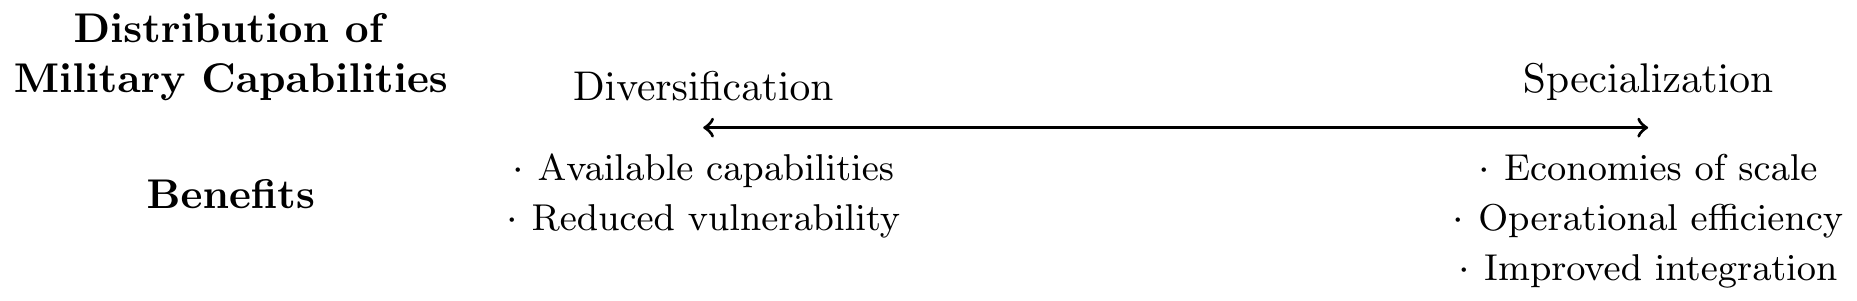
\includegraphics{2023-07-13_Specialization_files/figure-pdf/fig-spectrum_specialization-1.png}

}

\caption{\label{fig-spectrum_specialization}Varieties of a state's
distribution of military capabilities.}

\end{figure}

First, the cost of setting up manufacturing and acquiring the materials
for weapons acquisition entail large upfront investment. But the
marginal cost of that investment goes down as a state decides to produce
more of the same asset (Markowski and Hall 1998). For example, Germany
has reduced the need for redundant infrastructure by centralizing car
and light truck production all within the Bundeswehr-Fuhrparkservice
GmbH which allows them to produce newer but less varied vehicles more
quickly (Overhage 2013). Economies of scales are also ``active'' in that
they accrue as a state undertakes defense-related activities, so the
more a state operates with a particular asset, the lower their marginal
costs because of ``learning by doing'' (Postrel 2002). Even states that
are primarily ``arms buyers'' as opposed to ``arms builders'' experience
reduced maintenance and repair costs from a shorter list of components
and end-use products.\footnote{There are, of course, still differences
  in accrued economies of scale from indigenous production as opposed to
  purchasing foreign equipment for one's own military (Neuman 1994;
  Brooks 2005; DeVore 2011; von Hlatky and Rice 2018). Given the
  difficulty in acquiring large-scale data on the domestic producers of
  different component parts in multi-national arms production
  arrangements, this paper simply argues that there are some positive
  economies of scale in specialization, even for arms buyers, and leaves
  future research to identify the difference in degree across these two
  mechanisms of making versus buying.}

Second, specialization allows a military to perform select missions more
efficiently by streamlining logistics and reducing the overall cost of
learning how to use new equipment. Many assets require
capability-specific investments that involve a fixed cost. A state with
several dozen different types of aircraft will require more complex
pilot training than a state that only has to master the effective use of
a few types of aircraft. One source of NATO's debate over who should
send main battle tanks to Ukraine concerns Ukraine's familiarity with
how those more complex systems work; they could immediately operate T-72
tanks sent from Eastern Europe, but training and logistics for the US
Abrams tank would take months (Lanoszka and Becker 2023, 6--10).

Third, integration is easier as a country specializes since the
complexity of integrating numerous types of platforms with various roles
and responsibilities decreases. Even issues as fine-grained as the
software used in various pieces of equipment are sufficient impediments
to military operations that nations consider this issue carefully.
NATO's Standardization Agreement (STANAG), for example, ensure broad
fleet compatibility with the same fuel nozzle. In 2019, Jordan gave up
its Chinese-built CH-4 drone fleet because successful integration with
other platforms was going to require a costly overhaul of their entire
communications system (Penney 2020).

In contrast to specialization, the benefits of diversification concern
the security gains of a full-spectrum military that makes combined arms
warfare possible (Biddle 2005). States that engage in a full-spectrum
approach to warfare instead of specializing benefit from having more of
the capabilities needed to defend themselves because ``each weapon,
unit, and technique possesses a unique set of capabilities and
vulnerabilities. Taking full advantage of these military assets
increases the likelihood that an armed force will fulfill its mission''
(Millett, Murray, and Watman 1986, 52). No weapons system is perfect,
and the nature of warfare means weapons systems that excel at one aspect
of international conflict do so precisely because they lack other
abilities. Aerial bombers sacrifice maneuverability so that they have
carry a high payload. But more maneuverable aircraft like fighters
achieve the benefits of speed with lower ordinate payloads. Far from
just a tactical consideration, this diversification is a political and
strategic concern since higher-order state objectives like credibility,
effectiveness, and efficiency are advanced by military platforms in
varying and often zero-sum ways. ``Military specialization imposes
opportunity costs in terms of what a nation does well and where it must
compromise its capabilities. Choices about what to buy, and where and
how to field the nation's military might, then pose certain constraints
on political strategy'' (J. R. Lindsay and Gartzke 2022, 346).

Diversification also reduces vulnerability by making it more difficult
for the adversary to develop countermeasures. A state with a limited
variety of assets has given their adversary a shorter list of
capabilities they must be able to defeat to prevail in combat. Air
defense systems, for example, come in three different varieties;
surface-to-air missiles (SAM), anti-aircraft artillery (AAA), and
aircraft armed with air-to-air missiles (AAM). These systems all differ
in the altitudes they can target, stealth, reaction times, mobility, and
cost. In a 1940 testimony before the Senate Appropriations Committee,
General George Marshall noted the need for both aircraft and
anti-aircraft artillery because the former is an area system that excels
at searching while the latter is a point system designed to protect key
assets. When asked by Congress which was most important he said all of
them; ``the whole thing is interwoven\ldots all these matters have to be
given proper weight to get a well integrated and balanced whole''
(Hammel 2010). A state that has chosen to develop only one of these
capabilities might have more in quantity (scale economies) and quality
(operational efficiency and improved integration), but they are now
vulnerable to the development of new missiles and aircraft designed to
circumvent the strengths of their adversary's one air defense system
(Gartzke, Kaplow, and Mehta 2014, 484--85).

Former US Chairman of the Joint Chiefs of Staff Colin Powell (2010, 157)
described a diverse, full-spectrum force as involving the ability to
``prevail, quickly, and cheaply, in any and all forms of conflict''.
States that have not embraced this model have consequently suffered.
After the Yom Kippur war, Israel opted to specialize their military by
cutting artillery and mechanized infantry in favor of a shift to pure
armor-aircraft. This left them vulnerable to an anti-armor and
anti-aircraft attack that set them back in the early stages of the 1973
Arab-Israeli War. It was only after they reversed course that they were
able to defeat the Egyptian air defense systems (Herzog 2018). After
World War II, India's Naval Plan Paper (1947) made the case for a
``balanced naval task force'' which was later explained by Vice Admiral
Parry (1949) as a move to reduce India's vulnerability with a navy
``containing all types of ships and aircrafts, on the sea, over the sea,
and under the sea''.

\hypertarget{alliances-increase-the-expected-benefits-of-specialization}{%
\subsection{Alliances increase the expected benefits of
specialization}\label{alliances-increase-the-expected-benefits-of-specialization}}

Even well-resourced states experience difficulty excelling at all forms
of conflict simultaneously (D. R. Lake 2012, 91). Making priorities is
both a product of luxury and of necessity. An actor can overcome this
constrained optimization problem and minimize the trade-off between
diversification and specialization through security
cooperation.\footnote{This theory is derived from business organization
  research on inter-firm cooperation (Gulati, Nohria, and Zaheer 2000;
  Meier, Stephenson, and Perkowski 2019).} Working with partners allows
for individual functional specialization under the auspices of a broader
defense arrangement. A parsimonious way to think about this in the
international context is defense alliances, since they are an indication
of the two prerequisites for security cooperation with a committed
partner: (1) belief in a partner's willingness to play a role in
improving your well-being and (2) their ability to do so (Morrow 1994;
Leeds 2003).\footnote{These two conditions exist more generally for
  theoretical cooperation (Deutsch 1962). I choose the language
  ``well-being'' rather than ``security'' because this also applies to
  asymmetric alliances where instead of seeking protection, the dominant
  state may be seeking autonomy to advance pursuit of its preferred
  foreign policy outcomes (Morrow 1991, 907--9).} Specialization is thus
not a questionable prioritization of efficiency by states choosing to
forgo the security benefits of a diversified military, but instead a way
to get the best of both worlds made possible by architectures of
international cooperation.

Alliances increase the payoffs of military specialization in a few ways.
Having allies who you believe will come to your defense allows a state
to allocate resources toward non-security functions since defense
resources are aggregated. In spending less on your own militarily, you
can under-invest in certain capabilities that have high marginal
production cost at current levels. Practitioners have recognized how the
resource re-allocation benefits of alliances translate to focused
specialization. US Naval Rear Admiral M. E. Smith (2013) noted that by
having a cooperative approach, ``each nation can avoid duplication and
thereby reduce its proportional share of the expense. This
is\ldots about a focused and pragmatic approach to force allocation that
acknowledges allies' existing contributions. Countries could immediately
apply the freed resources to unique national missions.''

Second, the resource gains under cooperation are more than the sum of
their parts because of scale economies. Collective defense can be more
than the sum of its parts if specialized actor bring a smaller variety
of capabilities to the table, but more of them. Discussions in the US
about a `1,000 ship Navy' are predicated on precisely this model; ``a
voluntarily global maritime network that ties together the collective
capabilities of free nations to establish and maintain a dramatically
increased level of international security in the maritime domain''
(Morgan and Martoglio 2005). Similarly, the 2002 Prague Summit outlined
8 areas over which NATO states could try to specialize, which 2011
Chicago Summit advocated as ``certain countries should let go of certain
capabilities in order to create a more rational defence structure from a
Brussels perspective'' (Christiansson 2013, 181--86).\footnote{Auerswald
  and Saideman (2014, 229--33) also point out specialization can help
  individual states engage in cost-effective defense investments while
  maintaining an aggregate full-spectrum allied force, but are skeptical
  trust issues can be overcome.} This resulted in Czechia specializing
in CBRN defense, Denmark omitting submarines, the Baltic states
emphasizing cyber defense at the expense of fighter aircraft, and a
handful of states taking the lead on strategic airlift.

\emph{Hypothesis: Specialization of defense capabilities should increase
with the presence of militarily-capable defense allies.}

Alliances that vary in their structure and purpose will also vary in the
mechanism by which they incentivize specialization (Leeds, Mattes, and
Vogel 2009; Mattes 2012). Specialization may be the product of high
interest alignment resolving coordination problems or hierarchy reducing
the risk of opportunism coercively or contractually (Gannon 2021). But
theorizing the conditions under which some alliances are more or less
likely to induce specialization risks putting the cart before the horse
without initial evidence that alliances influence the composition of a
state's arms portfolio at all. Linking alliance membership with higher
military specialization is a necessary precursor, setting the foundation
for differentiating alliances based on the mechanisms by which
specialization occurs and which alliance members specialize in what.

In sum, force structures that omit useful defense capabilities and/or
overproduce others can occur when a state has opted to specialize its
military portfolio. A state is more willing to do so when the security
risks of specialization are no longer prohibitive; a condition made
possible by alliance relationships that resolve the constrained
optimization problem. Shared defense thus garners the security benefits
of capability aggregation posited by the neo-realists (Parent and Rosato
2015) as well as the economic benefits put forth by hierarchy theorists
(D. A. Lake 2001, 147--51).

\hypertarget{sec-empirics}{%
\section{Empirical analysis}\label{sec-empirics}}

\hypertarget{dependent-variable}{%
\subsection{Dependent variable}\label{dependent-variable}}

The dependent variable is the degree of specialization of a state's
distribution of military capabilities in a given year. A state's
distribution of military capabilities is defined here as the combination
of military equipment that could be used by a state during conflict.
This includes platforms like artillery, aircraft, naval vessels, armored
vehicles, satellites, and transport ships.\footnote{The data do not
  include munitions like single-use bombs or ammunition or firearms used
  by individual military personnel. Existing research has made similar
  distinctions in what military capabilities are examined
  cross-nationally (Brooks and Wohlforth 2016).} I choose these scope
conditions because military platforms are equipment that can be
deployed, that other nations are likely to observe, that could be used
to signal intent and resolve in a crisis without actual use, and that
are durable goods.\footnote{While platforms and capabilities are not
  synonymous, there are here categorized based on their role/mission
  which serves as a reasonable proxy for capabilities. For example,
  fighter aircraft differ from bomber aircraft in what they allow a
  state to do, and those differ yet still from transport or tanker
  aircraft.} The index is constructed using the rDMC dataset detailing
annual counts of 69 different military platforms across all states from
1970-2014 (Gannon 2023).

To measure military specialization at the country-year level, I create
an index quantifying the differences across states' distribution of
military capabilities identified as omissions and over-productions
relative to the neorealist baseline assumption that states behave as
like-units under anarchy and should consequently seek similarly diverse
military capabilities subject to resource constraints.\footnote{This
  assumption simply sets 0 as a common reference point for the index.
  Even if we accept the common wisdom that all states specialize to some
  degree given optimization towards the most salient threats, the index
  still provides a way to compare relative degrees of specialization
  across observations. I choose the neorealist assumption of
  full-spectrum convergence because even those who believe observing
  specialization is obvious and intuitive have no clear prior about the
  \emph{degree} of specialization we should expect to see.} Assume that
global defense in year \(t\) is composed of \(N\) countries and \(M\)
military technologies. I construct an \(n \times m\) interaction matrix
for each year \(t\) such that each row \(n\) is a country and each
column \(m\) is a technology. Each cell thus represents the observed
count of a given technology in that country-year's military.\footnote{I
  include all branches of state militaries, including paramilitary
  branches like coast guards, for consistency across observations and
  because many states use or could use paramilitary forces
  internationally, even if in a non-military capacity like disaster
  relief or quasi-military capacity like gray zone conflict (Morris
  2018; Gannon et al. 2023).} In aggregate, this can be represented as
\(d_j = \sum_{i=1}^{N}(p'_{ij}ln\frac{p'_{ij}}{q_i})\) where \(N\) is
the total number of countries in that year, \(p_{ij}\) is country
\(i\)'s possession of technology \(j\) divided by the total amount of
technologies \(j\), and \(q_i\) is the total number of technologies
possessed by country \(i\) divided by the total number of technologies
in the world.\footnote{This bipartite network structure is modeled after
  its use in ecological research (Alarcón, Waser, and Ollerton 2008).}

From this, I calculate the functional entropy of each country's military
using a trait-based similarity measure drawn from Rao's (1982) quadratic
entropy calculation of the average difference across technology
portfolios between each country and all other countries in a given year
weighting the technologies by their relative abundance. This calculates
the functional entropy of a country's military as:
\(R(p_i,D) = \sum_{k=1}^{S} \sum_{l=1}^{S} \sqrt{(p_k|i)} \sqrt{(p_k|j)} d_{kl}\)
where \(p_i=(p_1|i, …, p_k|i, …, p_S|i)\) is the vector of relative
technology abundance within country \(i\); \(S\) is the number of
technologies; \(D=(d_kl)\) is the matrix of functional dissimilarity
between the technologies, and \(d_kl\) is the functional dissimilarity
between countries \(k\) and \(l\) (Pavoine 2020).\footnote{As this
  measure of functional entropy is developed by Pavoine et al. (2017),
  its formula is provided verbatim. In the original statistical ecology
  application, this measure uses Hill (1973) numbers to measure the
  dissimilarity between biological species based on observed traits,
  accounting for the rarity of those traits.}

To provide some intuition, this measure of entropy calculates the degree
of surprise or unpredictability produced by the difference between the
amount of a military capability we expect a country to possess and what
that country actually possess. This prior expectation is based on the
distribution of technologies across all other states and within the
state in question, thus providing a relative and absolute measure. For
example, if most states possess, on average, twice as many transport
helicopters as they do transport aircraft, we would expect a state with
10 transport aircraft to have roughly 20 transport helicopters. But if
the state in question already possessed many more transport aircraft
than everyone else, we would update our expectation since we know a way
this quantity differs from other states and other capabilities. Our
expectation for transport helicopters can thus be \emph{re}-calibrated
based on (1) the number of transport aircraft this states possesses
relative to everyone else's transport aircraft, and (2) the number of
transport aircraft this state possesses relative its other capabilities.
If we now reproduce this method across all other capabilities, we get a
revised prior expectation for the capability in question - transport
helicopters. The closer the observed quantity is to our final
re-calibrated expectation, the less entropy the quantity produces, and
thus the lower the level of specialization since producing many more or
far fewer transport helicopters than the model expects are both
indications that the state has absolute and relative specialization by
omitting or over-producing that capability relative to intra-state and
interstate expectation.

Figure~\ref{fig-spec_scores} shows the distribution of this index across
all observations.\footnote{There is a small, statistically significant,
  positive temporal trend in specialization that is accounted for in the
  statistical model. Technology evolves dynamically, in this case maybe
  due to shifts away from high-quantity legacy systems towards
  high-quality expeditionary warfare systems (Terriff, Osinga, and
  Farrell 2010; Schnaubelt 2011).} Among the most specialized
observations are Japan after 2010 and the least specialized include the
Baltic states in the early 1990's. Given the number of destroyers and
offshore coastal ships Japan possesses, having almost no amphibious
ships is an unexpected form of naval specialization (in the entropic
sense). So while Japan may dominate in many military capabilities, that
does not mean its relative dominance is equal across the board. Even the
United States has specialized, with famously risky and consequential
under-productions including the lack of minesweepers during the 1984
Iran-Iraq Tanker War (DeVore 2009), nuclear, chemical, and biological
(NBC) reconnaissance vehicles at the start of the 2003 Iraq War (Geis
2013, 241--55), and icebreakers over the past two decades (Markowitz
2020, 77--78). Importantly, having a diversified military is not
synonymous with having a lot of everything. States can have very little
of everything, making them similarly \emph{in}capable across the
board.\footnote{Almost all states possess certain capabilities like
  light transport aircraft and search and rescue helicopters. This is
  consistent with accounts of basic infrastructure ensured by ``critical
  assets'' (Matláry and Østerud 2007) and identifies the importance of
  accounting for economic capacity to ensure the specialization index is
  not simply measuring the luxury of economic choice.}

\begin{figure}[h]

{\centering 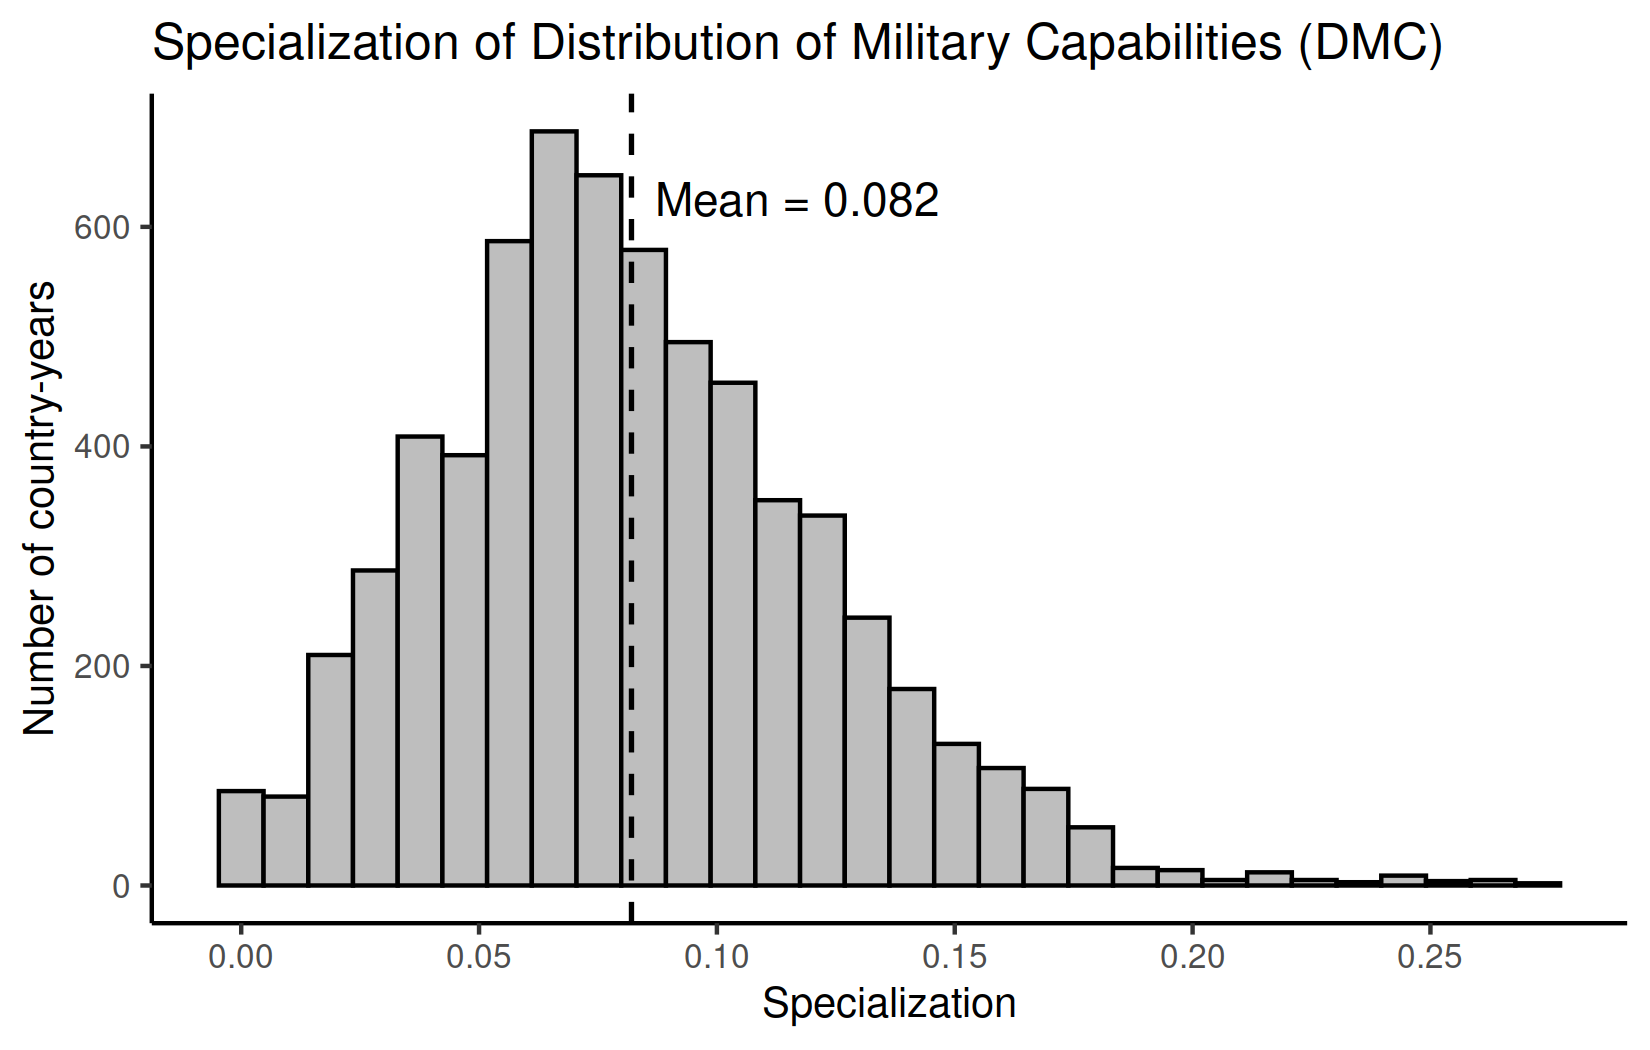
\includegraphics{2023-07-13_Specialization_files/figure-pdf/fig-spec_scores-1.png}

}

\caption{\label{fig-spec_scores}Distribution of country-year military
specialization. The measure is bounded between 0 and 1, with 1
representing the highest theoretically possible level of
specialization.}

\end{figure}

\hypertarget{independent-variable-and-controls}{%
\subsection{Independent variable and
controls}\label{independent-variable-and-controls}}

The independent variable measures a state's alliance
relationships.\footnote{Data on state participation in defensive
  alliance pacts is provided by the Alliance Treaty and Provisions
  (ATOP) dataset, version 5 (Leeds et al. 2002).} A state's allies are
those with whom it has a defensive alliance pact whereby the partner
state has made a promise to defend the state in question. As most states
have at least one formal treaty ally in a given year, existing research
using alliances as an independent variable has proxied for the
importance of a state's allies to that state's security. I
operationalize alliances at the country level two different ways; (1) as
the logged sum of military spending of a state's allies (excluding
itself) (DiGiuseppe and Poast 2016) and (2) the ratio between a state's
CINC score and the sum of their alliance CINC scores (including itself)
(Fang, Johnson, and Leeds 2014; Johnson, Leeds, and Wu 2015). For both
variables, higher values indicate more militarily-capable alliance
relationships which serves as an observable indicator of conditions
conducive to military specialization. Because a formal defense
commitment suggests a mutual belief in a partner's willingness and
ability to provide defense, a state with more militarily-capable allies
should be more confident that specializing its military will not leave
it vulnerable (A. Smith 1995; Benson and Clinton 2016).

I include a set of control variables that existing theories indicate
could be causally related to the dependent and/or independent variables
of interest. The models control for regime type, coding a country as a
democracy if they score higher than 6 on the 21-point Polity V index.
Democracies may spend less on defense (Fordham and Walker 2005), build
more capital-intensive militaries (Gartzke 2001), and be more
(DiGiuseppe and Poast 2016) or less (Gartzke and Gleditsch 2004)
reliable partners. There is also a control for whether a country has
been involved in an interstate war in the previous half decade, as a
salient threat environment (Ghosn, Palmer, and Bremer 2004) or recent
conflict experience may change patterns of innovation (Kollars 2015).
The models control for GDP, as resource-constrained states may be unable
to invest in a diverse array of military capital (Diehl 1994) or may
shift defense funds from platforms to personnel due to unemployment
(Becker 2021).\footnote{``Tech-flation'' could explain why higher
  security costs cause militaries to adopt fewer, but higher performing
  platforms (Adelman and Augustine 1990), although the empirical record
  in Europea suggests states diversify their military portfolios despite
  the financial cost of doing so (Howorth 2007).} Finally, I control for
CINC scores, as states harboring global ambitions may invest more in
power projection capabilities (Markowitz and Fariss 2018).\footnote{In
  addition to having unclear expectations about their relationship to
  specialization, time-invariant geographic variables are addressed via
  fixed effects models in the appendix rather than constant model
  parameters that risk model degeneration (Beck 2011).}

\hypertarget{model-and-results}{%
\subsection{Model and results}\label{model-and-results}}

The dependent variable is military specialization of country \(i\) in
year \(j\), measured with the functional entropy index described above.
Higher values indicate more specialization and less diversification. As
the dependent variable is continuous, I estimate a series of ordinary
least square (OLS) regressions using the two different independent
variables - (1) logged sum of allied military spending, (2) ratio of a
country's CINC score to that of all its allies and itself. For each
independent variable, I estimate a bivariate model country-clustered
standard errors to account for the non-independence between observations
in panel data (Cameron and Miller 2015) then a model that adds all
control variables and year scaled cubic polynomials to account for
temporal specialization trends (D. B. Carter and Signorino 2010).
Summary statistics for all model variables is provided in Appendix Table
A1.

I present the OLS results here as they are most easily interpretable and
consistent with modeling specifications in existing research with
similar data. Table~\ref{tbl-results} shows the results of all four
models. Models 1 and 2 demonstrate allied military spending is
positively associated with military specialization with statistical
significance of at least the 0.05 standardized level. Although allies'
CINC ratio is negative associated with military specialization in the
bivariate model (Model 3), the inclusion of control variables and
temporal dependencies (Model 4) reverses the association by minimizing
omitted variable bias, which is consistent with the other models and
theoretical expectations. In aggregate, these results provides
suggestive evidence that states that have militarily-capable alliance
partners have more specialized military portfolios - omitting certain
capabilities and over-producing other capabilities - relative to states
that are reliant upon self-defense.

Recognizing the non-random assignment of alliance membership as well as
a plausible endogeneous process whereby specialization makes alliance
membership more likely, we urge the reader to interpret these results as
consistent with theoretical expectations, rather than evidence of
causality. To minimize some of these concerns where possible, a series
of alternate model specifications are provided in the appendix that
relax assumptions about the underlying distribution of the dependent
variable and temporal and country-specific trends. The findings are
robust across alternate modeling parameters. Similar results are found
using fractional logit and beta regressions (Appendix Table A2),
Bayesian zero-inflated and ordered beta regressions (Appendix Table A3),
with alternate fixed effects and standard error clustering
specifications (Appendix Table A4), and using different controls like
operationalizing manufacturing base strength with GDP per capita instead
of GDP (Appendix Table A5). Nonetheless, quantitative models of
observational panel data are limited in their ability to address these
concerns, so further research should validate this claim qualitatively
by, for example, process tracing specialization in states before and
after joining an alliance like recent waves of NATO expansion.

\hypertarget{tbl-results}{}
\begin{table}
\caption{\label{tbl-results}Military Specialization and Alliances, Multivariate Analysis }\tabularnewline

\centering
\begin{tabular}[t]{lcccc}
\toprule
  & (1) & (2) & (3) & (4)\\
\midrule
Allies' Mil Spend. (log) & \num{0.004}*** & \num{0.001}* &  & \\
 & (\num{<0.001}) & (\num{0.035}) &  & \\
Allies' CINC Ratio &  &  & \num{-0.045}* & \num{0.025}*\\
 &  &  & (\num{0.022}) & (\num{0.035})\\
Democracy &  & \num{-0.002} &  & \num{0.000}\\
 &  & (\num{0.515}) &  & (\num{0.958})\\
Interstate War (5yr lag) &  & \num{0.001} &  & \num{0.002}\\
 &  & (\num{0.846}) &  & (\num{0.674})\\
GDP (log) &  & \num{0.012}*** &  & \num{0.013}***\\
 &  & (\num{<0.001}) &  & \vphantom{3} (\num{<0.001})\\
CINC &  & \num{0.183} &  & \num{0.203}\\
 &  & (\num{0.293}) &  & (\num{0.278})\\
Year &  & \num{0.006}*** &  & \num{0.006}***\\
 &  & (\num{<0.001}) &  & \vphantom{2} (\num{<0.001})\\
Year$^2$ &  & \num{0.000}*** &  & \num{0.000}***\\
 &  & (\num{<0.001}) &  & \vphantom{1} (\num{<0.001})\\
Year$^3$ &  & \num{0.000}*** &  & \num{0.000}***\\
 &  & (\num{<0.001}) &  & (\num{<0.001})\\
\midrule
Num.Obs. & \num{4629} & \num{3900} & \num{4568} & \num{3900}\\
AIC & \num{-7400.7} & \num{-9085.7} & \num{-7079.8} & \num{-9067.4}\\
BIC & \num{22397.6} & \num{15306.0} & \num{22265.1} & \num{15324.2}\\
\bottomrule
\multicolumn{5}{l}{\rule{0pt}{1em}+ p $<$ 0.1, * p $<$ 0.05, ** p $<$ 0.01, *** p $<$ 0.001}\\
\multicolumn{5}{l}{\textsuperscript{a} All models include country-clustered standard errors.}\\
\end{tabular}
\end{table}

The relationship between alliances and military specialization is also
substantively significant. Holding all control variables constant, a one
standard deviation increase in allies' CINC ratio (independent variable
in Models 3 and 4) is associated with a 1.4\% increase in a state's
military specialization; the difference in Japan's military
specialization between 1982 and 2000. Despite what what is traditionally
understood as a lopsided division of security responsibilities, the US
and Japan have each specialized their security responsibilities
intentionally (Ando 2015). Japan's 1982 capability realignment described
in Section~\ref{sec-intro} signaled the start of a new era of
cooperation with the United States, with the joint communique issued by
Prime Minister Suzuki and President Reagan (1981, 3) stressing ``the
desirability of an appropriate division of roles between Japan and the
United States''. Japan was entrusted with protecting its sea lines of
communication (SLOCs) 1,000 nautical miles off its coast and providing
logistical support to offensive US operations as needed.
Figure~\ref{fig-japan} illustrates how one result of this strengthened
alliance was a more specialized Japanese military. Japan doubled its SAM
and far-from-shore naval capabilities like destroyers and utility
helicopters and significantly downsized its amphibious and coastal
fleets. The alliance relationship with the United States allowed Japan
to carry the ``defensive shield'' by specializing in capabilities for
SLOCs and rear-area support while forgoing ``offensive spear''
attack-capable surface ships and high-tech long-range aircraft (Schoff
2014).\footnote{This case illustrates an important avenue for future
  research - the degree to which specialization at the dyad or
  alliance-level is complementary. An allies' defense portfolio can
  compensate for a given state's specialization by possessing the
  capabilities the given state is missing or by possessing a diversified
  full-spectrum force. The former suggests the reliance is
  unidirectional, while the latter suggests a degree of mutual
  interdependence.}

\begin{figure}[H]

{\centering 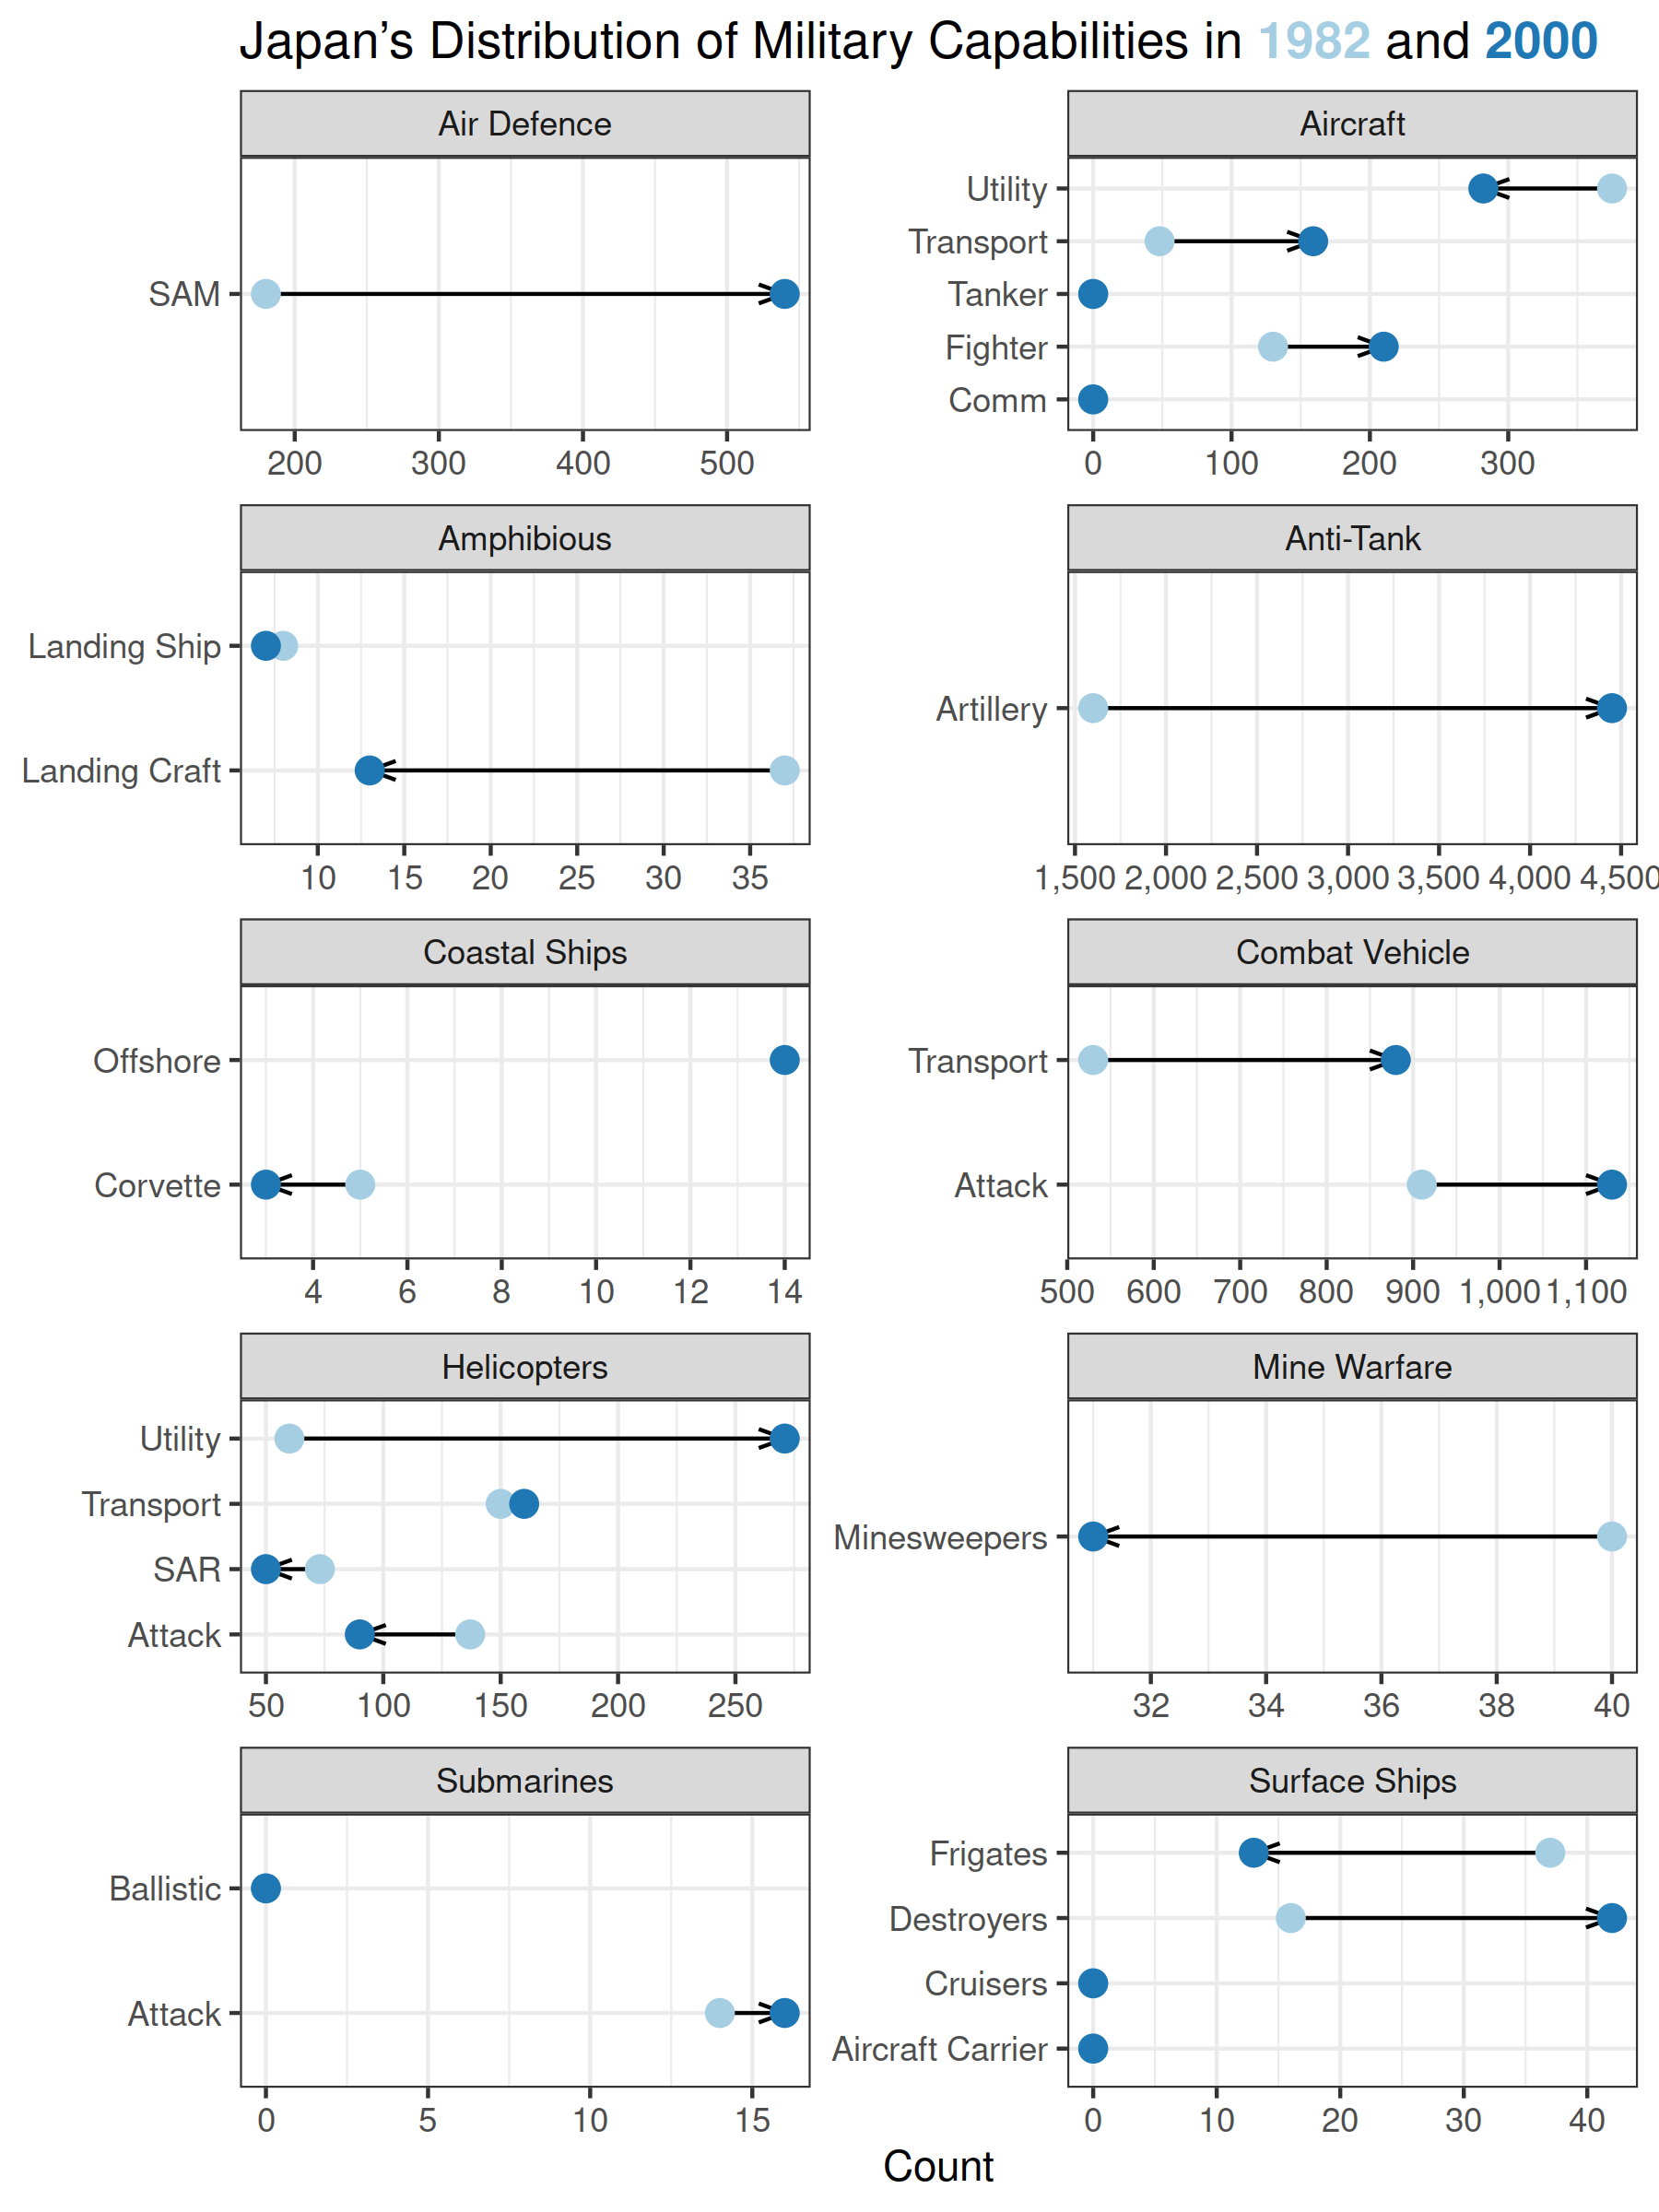
\includegraphics{2023-07-13_Specialization_files/figure-pdf/fig-japan-1.png}

}

\caption{\label{fig-japan}Change in Japan's distribution of military
capabilities between 1982 and 2000. Capabilities Japan did not possess
at any point during this time period (eg ballistic missiles and drones)
are omitted.}

\end{figure}

\hypertarget{sec-conclusion}{%
\section{Implications and avenues for future
research}\label{sec-conclusion}}

Variation in the composition of militaries across time and space is the
result of political decisions by states to spend defense dollars
dissimilarly (Kunertova 2017; Becker et al. 2022). This paper's two
central contributions concern identifying and explaining that, first in
precisely measuring one important dimension on which military portfolios
vary - their degree of specialization - and second in putting forth one
novel explanation for that variation - alliances.

By advancing discussion from burden-sharing \emph{costs} to
burden-sharing \emph{configurations}, new perspectives on the value of
alliances emerge. Contra neorealist pessimism about cooperation under
anarchy, relying on other states for your security is neither infrequent
nor inefficient. Specialization is evidence that relying on partners for
defense happens frequently since alliance participants more often accept
the risks of forgoing a diversified force and instead specialize in
capabilities seemingly ill-suited to their immediate security but
compatible with collective security. Doing so requires trust that
alliances allow them to gain the benefits of specialization and
diversification in ways they could not if providing for their security
alone.

Specialization also questions the inefficiency of external balancing, as
it explains a mechanism by which alliances provide ``greater security
with fewer resources but more coordination'' (Rasmussen 2011) in a way
that questions pessimistic accounts in ongoing debates about the
economic consequences of alliances (DiGiuseppe and Poast 2016; Alley and
Fuhrmann 2021; Cooley et al. 2022) and burden-sharing (Oneal and Diehl
1994; Blankenship 2021; Becker et al. 2023). Then US ambassador to NATO
Ivo Daalder (2013) noted that the problem was not that NATO countries
were not spending enough on defense, it was that they were not spending
that money wisely. In contextualizing the economic implications of
specialization and diversification to the defense portfolio context,
this paper provides a way to alleviate concerns that alliances are
nothing more than wasteful spending. Allies can turn to specialization
to ensure that spending is efficient while still being efficacious. As
UK Secretary of Defence Hammond (2012) explained, the answer to economic
pressure lies in ``prioritizing ruthlessly, specializing aggressively,
and collaborating unsentimentally.''

Far from just being a political economy story, this finding also has
important implications for national security. Efficiencies gained across
partners can mean more collective security per dollar. Rather than
redundancy across contributors, cooperating states can excel at their
particular cog in a collective security machine. Cooperation allows
states to ``take advantage of economies of scale in the provision of
defense and to benefit from specialization by coordinating training,
equipment, and procedures. By pooling their efforts and/or cooperating
with states that have different comparative advantages, leaders hope to
create a stronger joint fighting force'' (Leeds and Anac 2005, 185). But
specializing one's military because of reliance on others is not without
its risks, as there is always a ``fear that the other will not live up
to the terms of the agreement'' (D. A. Lake 1996, 15). Japan and South
Korea's defense strategies have remained neither static nor similar.
Contemporary discussions about militarization in response to Chinese,
North Korean, and Russian threat have put their respective alliances
with the US front and center (Katz, Johnstone, and Cha 2023). To the
degree that Japan has specialized their military in forgoing and/or
overemphasized certain capabilities because of their relationship with
the United States, their ability to defend themselves in the event of
attack may be compromised (Matsuda 2023). South Korea may be trending in
the opposite direction, signaling their discontent with the alliance by
publicly contemplating the need to duplicate uncertain US nuclear
protection with an arsenal of their own (Lind and Press 2023). More
generally, if states feel confident they can rely on their allies, we
should see them continue to specialize their militaries. Conversely,
allies beginning to diversifying their military portfolios may be
hedging their bets in seeking to defend themselves with a full-spectrum
force rather than risk the consequences of abandonment.

Future inquiries should explore several critical avenues. Defense
cooperation takes many governance forms that allow states to rely on
each other to different degrees and for different reasons (Benson 2012),
particularly if research extended to other time periods less dominated
by asymmetric and institutionalized alliances than the post-1970 period
analyzed here (Palmer and Souchet 1994). Differences across alliances in
joint war planning (Poast 2019a, 174--75), the threat environment (Niou
and Zeigler 2019), and degree of domination (Lanoszka 2013) may
influence who specializes in what and the degree to which specialization
by partners produces a coordinated and complementary division of labor
(Takabatake 2023). Future work could also look at the size of alliances
(Fordham and Poast 2016), specialization across issue areas like
diplomacy or economics (Kinne and Bunte 2020), or different kinds of
security alignments like defense cooperation agreements (DCAs) (Kinne
2020) and ad-hoc coalitions (Kreps 2011; Cappella Zielinski and Poast
2021).

Despite fear of exploitation being most salient where survival is at
stake, specialization is evidence states can manage uncertainty about
cooperation under anarchy by increasing its expected benefits. Even if
states do design their militaries primarily to deal with external
threats, this is conditioned by their alliance relationships in a way
that demonstrates novelty in the value of the latter. This does not
negate the conventional wisdom that militaries are primarily structured
to counter foreign threats, but it does question a common belief that
internal balancing and imitation - even in the face of a common enemy -
is the best form of defense in the self-help world of anarchy. One of
the very purposes of alliances is to change states' defense spending and
their military portfolio. Rather than think about arms and allies are
distinct strategies for security - one of which may be better than the
other - we should recognize that the arms a state develops are a
function of the arms of its allies.

\newpage

\hypertarget{references}{%
\section*{References}\label{references}}
\addcontentsline{toc}{section}{References}

\hypertarget{refs}{}
\begin{CSLReferences}{1}{0}
\leavevmode\vadjust pre{\hypertarget{ref-adelman_defenserevolutionstrategy_1990}{}}%
Adelman, Kenneth L., and Norman R. Augustine. 1990. \emph{The Defense
Revolution: Strategy for the Brave New World}. {San Francisco, Calif. :
Lanham, Md}: {ICS Press}.

\leavevmode\vadjust pre{\hypertarget{ref-alarcon_yeartoyearvariationtopology_2008}{}}%
Alarcón, Ruben, Nickolas M. Waser, and Jeff Ollerton. 2008.
{``Year-to-Year Variation in the Topology of a
Plant\textendash pollinator Interaction Network.''} \emph{Oikos} 117
(12): 1796--1807.
\url{https://doi.org/10.1111/j.0030-1299.2008.16987.x}.

\leavevmode\vadjust pre{\hypertarget{ref-alley_budgetbreakerfinancial_2021}{}}%
Alley, Joshua, and Matthew Fuhrmann. 2021. {``Budget {Breaker}? {The
Financial Cost} of {US Military Alliances}.''} \emph{Security Studies}
30 (5): 661--90. \url{https://doi.org/10.1080/09636412.2021.2021280}.

\leavevmode\vadjust pre{\hypertarget{ref-allison_armamentsarmscontrol_1975}{}}%
Allison, Graham T., and Frederic A. Morris. 1975. {``Armaments and {Arms
Control}: {Exploring} the {Determinants} of {Military Weapons}.''}
\emph{Daedalus} 104 (3): 99--129.
\url{https://www.jstor.org/stable/20024348}.

\leavevmode\vadjust pre{\hypertarget{ref-altfeld_decisionallytheory_1984}{}}%
Altfeld, Michael. 1984. {``The {Decision To Ally}: A {Theory} and
{Test}.''} \emph{Western Political Quarterly} 37 (4): 523--44.
\url{https://doi.org/10.1177/106591298403700402}.

\leavevmode\vadjust pre{\hypertarget{ref-ando_empiricalanalysisdefense_2015}{}}%
Ando, Shio. 2015. {``Empirical Analysis of the Defense Interdependence
Between {Japan} and the {United States}.''} \emph{Defence and Peace
Economics} 26 (2): 223--31.
\url{https://doi.org/10.1080/10242694.2013.793531}.

\leavevmode\vadjust pre{\hypertarget{ref-andzans_deterrencedilemmalatvia_2017}{}}%
Andžāns, Māris, and Viljar Veebel. 2017. {``Deterrence {Dilemma} in
{Latvia} and {Estonia}: {Finding} the {Balance} Between {External
Military Solidarity} and {Territorial Defence}.''} \emph{Journal on
Baltic Security} 3 (2): 29--41.

\leavevmode\vadjust pre{\hypertarget{ref-art_bureaucraticpoliticsamerican_1973}{}}%
Art, Robert J. 1973. {``Bureaucratic Politics and {American} Foreign
Policy: {A} Critique.''} \emph{Policy Sciences} 4 (4): 467--90.
\url{https://doi.org/10.1007/BF01728472}.

\leavevmode\vadjust pre{\hypertarget{ref-auerswald_natoafghanistanfighting_2014}{}}%
Auerswald, David, and Stephen Saideman. 2014. \emph{{NATO} in
{Afghanistan}: {Fighting Together}, {Fighting Alone}}. {Princeton, NJ}:
{Princeton University Press}.

\leavevmode\vadjust pre{\hypertarget{ref-beck_fixedeffectstimeinvariantvariables_2011}{}}%
Beck, Nathaniel. 2011. {``Of {Fixed-Effects} and {Time-Invariant
Variables}.''} \emph{Political Analysis} 19 (2): 119--22.
\url{https://www.jstor.org/stable/23011256}.

\leavevmode\vadjust pre{\hypertarget{ref-becker_rustygunsbuttery_2021}{}}%
Becker, Jordan. 2021. {``Rusty Guns and Buttery Soldiers: Unemployment
and the Domestic Origins of Defense Spending.''} \emph{European
Political Science Review} 13 (3): 307--30.
\url{https://doi.org/10.1017/S1755773921000102}.

\leavevmode\vadjust pre{\hypertarget{ref-becker_disaggregateddefensespending_2022}{}}%
Becker, Jordan, Seth Benson, John Paul Dunne, and Edmund J. Malesky.
2022. {``Disaggregated {Defense Spending}: {Introduction} to {Data} and
the {Case} for {Systematic Use}.''} \{\{SSRN Scholarly Paper\}\}.
{Rochester, NY}. \url{https://doi.org/10.2139/ssrn.4241307}.

\leavevmode\vadjust pre{\hypertarget{ref-becker_transatlanticshakedownpresidential_2023}{}}%
Becker, Jordan, Sarah E Kreps, Paul Poast, and Rochelle Terman. 2023.
{``Transatlantic {Shakedown}: {Presidential Shaming} and {NATO Burden
Sharing}.''} \emph{Journal of Conflict Resolution} 0 (0): 1--35.
\url{https://doi.org/10.1177/00220027231167840}.

\leavevmode\vadjust pre{\hypertarget{ref-beckley_powernationsmeasuring_2018}{}}%
Beckley, Michael. 2018. {``The {Power} of {Nations}: {Measuring What
Matters}.''} \emph{International Security} 43 (2): 7--44.
\url{https://doi.org/10.1162/isec_a_00328}.

\leavevmode\vadjust pre{\hypertarget{ref-benson_constructinginternationalsecurity_2012}{}}%
Benson, Brett V. 2012. \emph{Constructing {International Security}:
{Alliances}, {Deterrence}, and {Moral Hazard}}. {Cambridge University
Press}.

\leavevmode\vadjust pre{\hypertarget{ref-benson_assessingvariationformal_2016}{}}%
Benson, Brett V., and Joshua D. Clinton. 2016. {``Assessing the
{Variation} of {Formal Military Alliances}.''} \emph{Journal of Conflict
Resolution} 60 (5): 866--98.
\url{https://doi.org/10.1177/0022002714560348}.

\leavevmode\vadjust pre{\hypertarget{ref-betts_shouldstrategicstudies_1997}{}}%
Betts, Richard K. 1997. {``Should {Strategic Studies Survive}?''}
\emph{World Politics} 50 (1): 7--33.
\url{https://doi.org/10.1017/S0043887100014702}.

\leavevmode\vadjust pre{\hypertarget{ref-biddle_militarypowerexplaining_2005}{}}%
Biddle, Stephen. 2005. \emph{Military {Power}: {Explaining Victory} and
{Defeat} in {Modern Battle}}. {Manas Publications}.

\leavevmode\vadjust pre{\hypertarget{ref-blankenship_priceprotectionexplaining_2021}{}}%
Blankenship, Brian. 2021. {``The {Price} of {Protection}: {Explaining
Success} and {Failure} of {US Alliance Burden-Sharing Pressure}.''}
\emph{Security Studies} 30 (5): 691--724.
\url{https://doi.org/10.1080/09636412.2021.2018624}.

\leavevmode\vadjust pre{\hypertarget{ref-brooks_producingsecuritymultinational_2005}{}}%
Brooks, Stephen G. 2005. \emph{Producing {Security}: {Multinational
Corporations}, {Globalization}, and the {Changing Calculus} of
{Conflict}}. {Princeton University Press}.
\url{https://www.jstor.org/stable/j.ctt7sjz7}.

\leavevmode\vadjust pre{\hypertarget{ref-brooks_risefallgreat_2016}{}}%
Brooks, Stephen G., and William C. Wohlforth. 2016. {``The {Rise} and
{Fall} of the {Great Powers} in the {Twenty-first Century}: {China}'s
{Rise} and the {Fate} of {America}'s {Global Position}.''}
\emph{International Security} 40 (3): 7--53.
\url{https://doi.org/10.1162/ISEC_a_00225}.

\leavevmode\vadjust pre{\hypertarget{ref-brzoska_reportingmilitaryexpenditures_1981}{}}%
Brzoska, Michael. 1981. {``The Reporting of Military Expenditures.''}
\emph{Journal of Peace Research} 18 (3): 261--75.

\leavevmode\vadjust pre{\hypertarget{ref-buzan_introductionstrategicstudies_1987}{}}%
Buzan, Barry. 1987. \emph{An {Introduction} to {Strategic Studies}:
{Military Technology} and {International Relations}}. {London}:
{Springer}.

\leavevmode\vadjust pre{\hypertarget{ref-buzan_logicanarchyneorealism_1993}{}}%
Buzan, Barry, Charles A. Jones, and Richard Little. 1993. \emph{The
{Logic} of {Anarchy}: {Neorealism} to {Structural Realism}}. {New York}:
{Columbia University Press}.

\leavevmode\vadjust pre{\hypertarget{ref-cameron_practitionerguideclusterrobust_2015}{}}%
Cameron, A. Colin, and Douglas L. Miller. 2015. {``A {Practitioner}'s
{Guide} to {Cluster-Robust Inference}.''} \emph{Journal of Human
Resources} 50 (2): 317--72. \url{https://doi.org/10.3368/jhr.50.2.317}.

\leavevmode\vadjust pre{\hypertarget{ref-cappellazielinski_supplyingalliespolitical_2021}{}}%
Cappella Zielinski, Rosella, and Paul Poast. 2021. {``Supplying
{Allies}: {Political Economy} of {Coalition Warfare}.''} \emph{Journal
of Global Security Studies} 6 (1).
\url{https://doi.org/10.1093/jogss/ogaa006}.

\leavevmode\vadjust pre{\hypertarget{ref-carroll_predictionproxiespower_2019}{}}%
Carroll, Robert J., and Brenton Kenkel. 2019. {``Prediction, {Proxies},
and {Power}.''} \emph{American Journal of Political Science} 63 (3):
577--93. \url{https://doi.org/10.1111/ajps.12442}.

\leavevmode\vadjust pre{\hypertarget{ref-carter_backfuturemodeling_2010}{}}%
Carter, David B., and Curtis S. Signorino. 2010. {``Back to the
{Future}: {Modeling Time Dependence} in {Binary Data}.''}
\emph{Political Analysis} 18 (3): 271--92.
\url{https://doi.org/10.1093/pan/mpq013}.

\leavevmode\vadjust pre{\hypertarget{ref-carter_senatedefensebudgeting_1989}{}}%
Carter, Ralph G. 1989. {``Senate {Defense Budgeting}, 1981-1988: {The
Impacts} of {Ideology}, {Party}, and {Constituency Benefit} on the
{Decision} to {Support} the {President}.''} \emph{American Politics
Quarterly} 17 (3): 332--47.
\url{https://doi.org/10.1177/1532673X8901700306}.

\leavevmode\vadjust pre{\hypertarget{ref-caverley_unitedstateshegemony_2007}{}}%
Caverley, Jonathan D. 2007. {``United {States Hegemony} and the {New
Economics} of {Defense}.''} \emph{Security Studies} 16 (4): 598--614.
\url{https://doi.org/10.1080/09636410701740825}.

\leavevmode\vadjust pre{\hypertarget{ref-christiansson_poolingsharingspecializing_2013}{}}%
Christiansson, Magnus. 2013. {``Pooling, {Sharing} and {Specializing}
\textemdash{} {NATO} and {International Defence Cooperation}.''} In
\emph{{NATO} Beyond 9/11: {The Transformation} of the {Atlantic
Alliance}}, edited by Ellen Hallams, Luca Ratti, and Benjamin Zyla,
178--97. New {Security Challenges}. {London}: {Palgrave Macmillan UK}.
\url{https://doi.org/10.1057/9780230391222_9}.

\leavevmode\vadjust pre{\hypertarget{ref-conybeare_armsalliancescapital_1994}{}}%
Conybeare, John A. C. 1994. {``Arms {Versus Alliances}: {The Capital
Structure} of {Military Enterprise}.''} \emph{Journal of Conflict
Resolution} 38 (2): 215--35.
\url{https://doi.org/10.1177/0022002794038002003}.

\leavevmode\vadjust pre{\hypertarget{ref-cooley_estimatingalliancecosts_2022}{}}%
Cooley, Alexander, Daniel H. Nexon, Paul Poast, Joshua Alley, and
Matthew Fuhrmann. 2022. {``Estimating {Alliance Costs}: {An
Exchange}.''} \emph{Security Studies} 31 (3): 510--32.
\url{https://doi.org/10.1080/09636412.2022.2101324}.

\leavevmode\vadjust pre{\hypertarget{ref-crisher_powernationalcapability_2017}{}}%
Crisher, Brian. 2017. {``Power and {National Capability}.''} In
\emph{Oxford {Research Encyclopedia} of {Politics}}. {Oxford University
Press}. \url{https://doi.org/10.1093/acrefore/9780190228637.013.468}.

\leavevmode\vadjust pre{\hypertarget{ref-daalder_renewedambitionsnato_2013}{}}%
Daalder, Ivo. 2013. {``Renewed {Ambitions} for {NATO}.''}

\leavevmode\vadjust pre{\hypertarget{ref-deudney_bindingsovereignsauthorities_1996}{}}%
Deudney, Daniel. 1996. {``Binding {Sovereigns}: {Authorities},
{Structures}, and {Geopolitics} in {Philadelphian Systems}.''} In
\emph{State {Sovereignty} as {Social Construct}}, edited by Thomas J.
Biersteker and Cynthia Weber, 190--239. {Cambridge University Press}.

\leavevmode\vadjust pre{\hypertarget{ref-deutsch_cooperationtrusttheoretical_1962}{}}%
Deutsch, Morton. 1962. {``Cooperation and Trust: {Some} Theoretical
Notes.''} In \emph{Nebraska {Symposium} on {Motivation}, 1962},
275--320. {Oxford, England}: {Univer. Nebraska Press}.

\leavevmode\vadjust pre{\hypertarget{ref-devore_convenientframeworkwestern_2009}{}}%
DeVore, Marc R. 2009. {``A Convenient Framework: The {Western European
Union} in the {Persian Gulf}, 1987\textendash 1988 and
1990\textendash 1991.''} \emph{European Security} 18 (2): 227--43.
\url{https://doi.org/10.1080/09662830903460087}.

\leavevmode\vadjust pre{\hypertarget{ref-devore_armscollaborationdilemma_2011}{}}%
---------. 2011. {``The {Arms Collaboration Dilemma}: {Between
Principal-Agent Dynamics} and {Collective Action Problems}.''}
\emph{Security Studies} 20 (4): 624--62.
\url{https://doi.org/10.1080/09636412.2011.625763}.

\leavevmode\vadjust pre{\hypertarget{ref-diehl_substitutescomplementseffects_1994}{}}%
Diehl, Paul F. 1994. {``Substitutes or Complements?: {The} Effects of
Alliances on Military Spending in Major Power Rivalries.''}
\emph{International Interactions} 19 (3): 159--76.
\url{https://doi.org/10.1080/03050629408434825}.

\leavevmode\vadjust pre{\hypertarget{ref-digiuseppe_armsdemocraticallies_2016}{}}%
DiGiuseppe, Matthew, and Paul Poast. 2016. {``Arms Versus {Democratic
Allies}.''} \emph{British Journal of Political Science} 48 (4):
981--1003. \url{https://doi.org/10.1017/S0007123416000247}.

\leavevmode\vadjust pre{\hypertarget{ref-downs_goodnewscompliance_1996}{}}%
Downs, George W., David M. Rocke, and Peter N. Barsoom. 1996. {``Is the
Good News about Compliance Good News about Cooperation?''}
\emph{International Organization} 50 (3): 379--406.
\url{https://doi.org/10.1017/S0020818300033427}.

\leavevmode\vadjust pre{\hypertarget{ref-edstrom_eaglebearexplaining_2020}{}}%
Edström, Håkan, and Jacob Westberg. 2020. {``Between the Eagle and the
Bear: {Explaining} the Alignment Strategies of the {Nordic} Countries in
the 21st Century.''} \emph{Comparative Strategy} 39 (2): 191--208.
\url{https://doi.org/10.1080/01495933.2020.1718994}.

\leavevmode\vadjust pre{\hypertarget{ref-elman_foreignpoliciessmall_1995}{}}%
Elman, Miriam Fendius. 1995. {``The {Foreign Policies} of {Small
States}: {Challenging Neorealism} in {Its Own Backyard}.''}
\emph{British Journal of Political Science} 25 (2): 171--217.
\url{https://www.jstor.org/stable/194084}.

\leavevmode\vadjust pre{\hypertarget{ref-evangelista_innovationarmsrace_1988}{}}%
Evangelista, Matthew A. 1988. \emph{Innovation and the {Arms Race}:
{How} the {United States} and the {Soviet Union Develop New Military
Technologies}}. {Ithaca, NY/London}: {Cornell University Press}.

\leavevmode\vadjust pre{\hypertarget{ref-eyre_statusnormsproliferation_1996}{}}%
Eyre, Dana P., and Mark C. Suchman. 1996. {``Status, {Norms} and the
{Proliferation} of {Conventional Weapons}: {An Institutional Theory
Approach}.''} In \emph{The {Culture} of {National Security}: {Norms} and
{Identity} in {World Politics}}, edited by Peter J. Katzenstein,
79--113. {New York, NY}: {Columbia University Press}.

\leavevmode\vadjust pre{\hypertarget{ref-fang_concederesistrestraining_2014}{}}%
Fang, Songying, Jesse C. Johnson, and Brett Ashley Leeds. 2014. {``To
{Concede} or to {Resist}? {The Restraining Effect} of {Military
Alliances}.''} \emph{International Organization} 68 (4): 775--809.
\url{https://doi.org/10.1017/S0020818314000137}.

\leavevmode\vadjust pre{\hypertarget{ref-farrell_weaponscausepolitics_1997}{}}%
Farrell, Theo. 1997. \emph{Weapons {Without} a {Cause}: {The Politics}
of {Weapons Acquisition} in the {United States}}. {London}: {St.
Martin's Press}.

\leavevmode\vadjust pre{\hypertarget{ref-fevolden_defenceindustrialpolicy_2016}{}}%
Fevolden, Arne Martin, and Kari Tvetbråten. 2016. {``Defence Industrial
Policy \textendash{} a Sound Security Strategy or an Economic
Fallacy?''} \emph{Defence Studies} 16 (2): 176--92.
\url{https://doi.org/10.1080/14702436.2016.1169893}.

\leavevmode\vadjust pre{\hypertarget{ref-fordham_domesticpoliticsworld_2019}{}}%
Fordham, Benjamin O. 2019. {``The {Domestic Politics} of {World Power}:
{Explaining Debates} over the {United States Battleship Fleet},
1890\textendash 91.''} \emph{International Organization} 73 (2):
435--68. \url{https://doi.org/10.1017/S0020818318000449}.

\leavevmode\vadjust pre{\hypertarget{ref-fordham_allalliancesare_2016}{}}%
Fordham, Benjamin O., and Paul Poast. 2016. {``All {Alliances Are
Multilateral}: {Rethinking Alliance Formation}.''} \emph{Journal of
Conflict Resolution} 60 (5): 840--65.
\url{https://doi.org/10.1177/0022002714553108}.

\leavevmode\vadjust pre{\hypertarget{ref-fordham_kantianliberalismregime_2005}{}}%
Fordham, Benjamin O., and Thomas C. Walker. 2005. {``Kantian
{Liberalism}, {Regime Type}, and {Military Resource Allocation}: {Do
Democracies Spend Less}?''} \emph{International Studies Quarterly} 49
(1): 141--57. \url{https://www.jstor.org/stable/3693628}.

\leavevmode\vadjust pre{\hypertarget{ref-gannon_usetheirforce_2021}{}}%
Gannon, J Andrés. 2021. {``Use {Their Force}: {Interstate Security
Alignments} and the {Distribution} of {Military Capabilities}.''} PhD
thesis, UC San Diego.

\leavevmode\vadjust pre{\hypertarget{ref-gannon_planestrainsarmored_2023}{}}%
---------. 2023. {``Planes, {Trains}, and {Armored Mobiles}:
{Introducing} a {Dataset} of the {Global Distribution} of {Military
Capabilities} ({rDMC}).''} \emph{International Studies Quarterly} 0 (0):
1--32. \url{https://doi.org/10.2139/ssrn.3930390}.

\leavevmode\vadjust pre{\hypertarget{ref-gannon_shadowdeterrencewhy_2023}{}}%
Gannon, J Andrés, Erik Gartzke, Jon R. Lindsay, and Peter Schram. 2023.
{``The {Shadow} of {Deterrence}: {Why Capable Actors Engage} in
{Contests Short} of {War}.''} \emph{Journal of Conflict Resolution},
April. \url{https://doi.org/10.1177/00220027231166345}.

\leavevmode\vadjust pre{\hypertarget{ref-gartzke_democracypreparationwar_2001}{}}%
Gartzke, Erik A. 2001. {``Democracy and the {Preparation} for {War}:
{Does Regime Type Affect States}' {Anticipation} of {Casualties}?''}
\emph{International Studies Quarterly} 45 (3): 467--84.
\url{https://doi.org/10.1111/0020-8833.00210}.

\leavevmode\vadjust pre{\hypertarget{ref-gartzke_whydemocraciesmay_2004}{}}%
Gartzke, Erik A., and Kristian Skrede Gleditsch. 2004. {``Why
{Democracies May Actually Be Less Reliable Allies}.''} \emph{American
Journal of Political Science} 48 (4): 775--95.
\url{https://doi.org/10.1111/j.0092-5853.2004.00101.x}.

\leavevmode\vadjust pre{\hypertarget{ref-gartzke_determinantsnuclearforce_2014}{}}%
Gartzke, Erik A., Jeffrey M. Kaplow, and Rupal N. Mehta. 2014. {``The
{Determinants} of {Nuclear Force Structure}.''} \emph{Journal of
Conflict Resolution} 58 (3): 481--508.
\url{https://doi.org/10.1177/0022002713509054}.

\leavevmode\vadjust pre{\hypertarget{ref-geis_burdensshadowsfuture_2013}{}}%
Geis, Anna. 2013. {``Burdens of the Past, Shadows of the Future: The Use
of Military Force as a Challenge for the {German} {`Civilian Power'}.''}
In \emph{The {Militant Face} of {Democracy}: {Liberal Forces} for
{Good}}, edited by Anna Geis, Harald Müller, and Niklas Schörnig,
231--68. {Cambridge University Press}.

\leavevmode\vadjust pre{\hypertarget{ref-ghosn_mid3dataset_2004}{}}%
Ghosn, Faten, Glenn Palmer, and Stuart A. Bremer. 2004. {``The {Mid3
Data Set}, 1993\textendash 2001: {Procedures}, {Coding Rules}, and
{Description}.''} \emph{Conflict Management and Peace Science} 21 (2):
133--54. \url{https://doi.org/10.1080/07388940490463861}.

\leavevmode\vadjust pre{\hypertarget{ref-goldman_systemiceffectsmilitary_1999}{}}%
Goldman, Emily O., and Richard B. Andres. 1999. {``Systemic Effects of
Military Innovation and Diffusion.''} \emph{Security Studies} 8 (4):
79--125. \url{https://doi.org/10.1080/09636419908429387}.

\leavevmode\vadjust pre{\hypertarget{ref-gulati_strategicnetworks_2000}{}}%
Gulati, Ranjay, Nitin Nohria, and Akbar Zaheer. 2000. {``Strategic
Networks.''} \emph{Strategic Management Journal} 21 (3): 203--15.
\url{https://doi.org/10.1002/(SICI)1097-0266(200003)21:3\%3C203::AID-SMJ102\%3E3.0.CO;2-K}.

\leavevmode\vadjust pre{\hypertarget{ref-halperin_bureaucraticpoliticsforeign_1974}{}}%
Halperin, Morton H., Priscilla Clapp, and Arnold Kanter. 1974.
\emph{Bureaucratic {Politics} and {Foreign Policy}}. {Washington DC}:
{Brookings Institution}.

\leavevmode\vadjust pre{\hypertarget{ref-hammel_roadbigweek_2010}{}}%
Hammel, Eric. 2010. \emph{The {Road} to {Big Week}: {The Struggle} for
{Daylight Air Supremacy Over Western Europe}, {July} 1942 \textendash{}
{February} 1944}. {Pacifica, CA}: {Pacifica Military History}.

\leavevmode\vadjust pre{\hypertarget{ref-hammond_natocasecollective_2012}{}}%
Hammond, Philip. 2012. {``{NATO}: {The} Case for Collective Defence in
the 21st {Century}.''} Speech. {The Atlantic Council}.

\leavevmode\vadjust pre{\hypertarget{ref-hendrickson_albanianatoopen_2006}{}}%
Hendrickson, Ryan C., Jonathan Campbell, and Nicholas Mullikin. 2006.
{``Albania and {NATO}'s {`{Open Door}'} {Policy}: {Alliance Enlargement}
and {Military Transformation}.''} \emph{The Journal of Slavic Military
Studies} 19 (2): 243--57.
\url{https://doi.org/10.1080/13518040600697779}.

\leavevmode\vadjust pre{\hypertarget{ref-herzog_waratonementstory_2018}{}}%
Herzog, Chaim. 2018. \emph{The {War} of {Atonement}: {The Inside Story}
of the {Yom Kippur War}}. {New York}: {Simon and Schuster}.

\leavevmode\vadjust pre{\hypertarget{ref-higgs_hardcoalsmake_1988}{}}%
Higgs, Robert. 1988. {``Hard {Coals Make Bad Law}: {Congressional
Parochialism} Versus {National Defense}.''} \emph{Cato Journal} 8 (1):
79--106.

\leavevmode\vadjust pre{\hypertarget{ref-hill_diversityevennessunifying_1973}{}}%
Hill, M. O. 1973. {``Diversity and {Evenness}: {A Unifying Notation} and
{Its Consequences}.''} \emph{Ecology} 54 (2): 427--32.
\url{https://doi.org/10.2307/1934352}.

\leavevmode\vadjust pre{\hypertarget{ref-hintz_symbolicamplificationsuboptimal_2022}{}}%
Hintz, Lisel, and David E. Banks. 2022. {``Symbolic {Amplification} and
{Suboptimal Weapons Procurement}: {Explaining Turkey}'s {S-400
Program}.''} \emph{Security Studies} 31 (5): 826--56.
\url{https://doi.org/10.1080/09636412.2022.2153733}.

\leavevmode\vadjust pre{\hypertarget{ref-horowitz_diffusionmilitarypower_2010}{}}%
Horowitz, Michael C. 2010. \emph{The {Diffusion} of {Military Power}:
{Causes} and {Consequences} for {International Politics}}. {Princeton
University Press}.

\leavevmode\vadjust pre{\hypertarget{ref-howorth_securitydefencepolicy_2007}{}}%
Howorth, Jolyon. 2007. \emph{The {Security} and {Defence Policy} in the
{European Union}}. {Palgrave Macmillan}.

\leavevmode\vadjust pre{\hypertarget{ref-johnson_capabilitycredibilityextended_2015}{}}%
Johnson, Jesse C., Brett Ashley Leeds, and Ahra Wu. 2015. {``Capability,
{Credibility}, and {Extended General Deterrence}.''} \emph{International
Interactions} 41 (2): 309--36.
\url{https://doi.org/10.1080/03050629.2015.982115}.

\leavevmode\vadjust pre{\hypertarget{ref-kadera_measuringnationalpower_2004}{}}%
Kadera, Kelly, and Gerald Sorokin. 2004. {``Measuring {National
Power}.''} \emph{International Interactions} 30 (3): 211--30.
\url{https://doi.org/10.1080/03050620490492097}.

\leavevmode\vadjust pre{\hypertarget{ref-katz_americaneedsreassure_2023}{}}%
Katz, Katrin Fraser, Christopher Johnstone, and Victor Cha. 2023.
{``America {Needs} to {Reassure Japan} and {South Korea}.''}
\emph{Foreign Affairs}, February.

\leavevmode\vadjust pre{\hypertarget{ref-kehr_battleshipbuildingparty_1975}{}}%
Kehr, Eckart. 1975. \emph{Battleship {Building} and {Party Politics} in
{Germany}, 1894-1901: {A Cross-section} of the {Political}, {Social} and
{Ideological Preconditions} of {German Imperialism}}. {University of
Chicago Press}.

\leavevmode\vadjust pre{\hypertarget{ref-kim_comparingmeasuresnational_2010}{}}%
Kim, Hyung Min. 2010. {``Comparing {Measures} of {National Power}.''}
\emph{International Political Science Review} 31 (4): 405--27.
\url{https://doi.org/10.1177/0192512110371239}.

\leavevmode\vadjust pre{\hypertarget{ref-kinne_defensecooperationagreement_2020}{}}%
Kinne, Brandon J. 2020. {``The {Defense Cooperation Agreement Dataset}
({DCAD}).''} \emph{Journal of Conflict Resolution} 64 (4): 729--55.
\url{https://doi.org/10.1177/0022002719857796}.

\leavevmode\vadjust pre{\hypertarget{ref-kinne_gunsmoneydefense_2020}{}}%
Kinne, Brandon J., and Jonas B. Bunte. 2020. {``Guns or {Money}?
{Defense Co-operation} and {Bilateral Lending} as {Coevolving
Networks}.''} \emph{British Journal of Political Science} 50 (3):
1067--88. \url{https://doi.org/10.1017/S0007123418000030}.

\leavevmode\vadjust pre{\hypertarget{ref-kinne_freeridingnetwork_2023}{}}%
Kinne, Brandon J., and Stephanie N. Kang. 2023. {``Free {Riding},
{Network Effects}, and {Burden Sharing} in {Defense Cooperation
Networks}.''} \emph{International Organization} 77 (2): 405--39.
\url{https://doi.org/10.1017/S0020818322000315}.

\leavevmode\vadjust pre{\hypertarget{ref-kollars_warhorizonsoldierled_2015}{}}%
Kollars, Nina A. 2015. {``War's {Horizon}: {Soldier-Led Adaptation} in
{Iraq} and {Vietnam}.''} \emph{Journal of Strategic Studies} 38 (4):
529--53. \url{https://doi.org/10.1080/01402390.2014.971947}.

\leavevmode\vadjust pre{\hypertarget{ref-kreps_coalitionsconvenienceunited_2011}{}}%
Kreps, Sarah. 2011. \emph{Coalitions of {Convenience}: {United States
Military Interventions} After the {Cold War}}. {Oxford University
Press}.

\leavevmode\vadjust pre{\hypertarget{ref-kunertova_onemeasurecannot_2017}{}}%
Kunertova, Dominika. 2017. {``One Measure Cannot Trump It All: Lessons
from {NATO}'s Early Burden-Sharing Debates.''} \emph{European Security}
26 (4): 552--74. \url{https://doi.org/10.1080/09662839.2017.1353495}.

\leavevmode\vadjust pre{\hypertarget{ref-kurth_whywebuy_1973}{}}%
Kurth, James R. 1973. {``Why {We Buy} the {Weapons We Do}.''}
\emph{Foreign Policy} 0 (11): 33--56.
\url{https://doi.org/10.2307/1148035}.

\leavevmode\vadjust pre{\hypertarget{ref-lake_technologyqualitativesuperiority_2012}{}}%
Lake, Daniel R. 2012. {``Technology, {Qualitative Superiority}, and the
{Overstretched American Military}.''} \emph{Strategic Studies Quarterly}
6 (4): 71--99.

\leavevmode\vadjust pre{\hypertarget{ref-lake_anarchyhierarchyvariety_1996}{}}%
Lake, David A. 1996. {``Anarchy, {Hierarchy}, and the {Variety} of
{International Relations}.''} \emph{International Organization} 50 (1):
1--33. \url{https://www.jstor.org/stable/2706997}.

\leavevmode\vadjust pre{\hypertarget{ref-lake_anarchyimportancesecurity_2001}{}}%
---------. 2001. {``Beyond {Anarchy}: {The Importance} of {Security
Institutions}.''} \emph{International Security} 26 (1): 129--60.
\url{https://doi.org/10.1162/016228801753212877}.

\leavevmode\vadjust pre{\hypertarget{ref-lake_newsovereigntyinternational_2003}{}}%
---------. 2003. {``The {New Sovereignty} in {International
Relations}.''} \emph{International Studies Review} 5 (3): 303--23.
\url{https://www.jstor.org/stable/3186572}.

\leavevmode\vadjust pre{\hypertarget{ref-lake_escapestatenature_2007}{}}%
---------. 2007. {``Escape from the {State} of {Nature}: {Authority} and
{Hierarchy} in {World Politics}.''} \emph{International Security} 32
(1): 47--79. \url{https://doi.org/10.1162/isec.2007.32.1.47}.

\leavevmode\vadjust pre{\hypertarget{ref-lanoszka_consentcoercionusing_2013}{}}%
Lanoszka, Alexander. 2013. {``Beyond Consent and Coercion: Using
Republican Political Theory to Understand International Hierarchies.''}
\emph{International Theory} 5 (3): 382--413.
\url{https://doi.org/10.1017/S1752971913000249}.

\leavevmode\vadjust pre{\hypertarget{ref-lanoszka_artpartialcommitment_2023}{}}%
Lanoszka, Alexander, and Jordan Becker. 2023. {``The Art of Partial
Commitment: The Politics of Military Assistance to {Ukraine}.''}
\emph{Post-Soviet Affairs} 39 (3): 173--94.
\url{https://doi.org/10.1080/1060586X.2022.2162758}.

\leavevmode\vadjust pre{\hypertarget{ref-lebovic_usingmilitaryspending_1999}{}}%
Lebovic, James H. 1999. {``Using {Military Spending Data}: {The
Complexity} of {Simple Inference}.''} \emph{Journal of Peace Research}
36 (6): 681--97. \url{https://doi.org/10.1177/0022343399036006005}.

\leavevmode\vadjust pre{\hypertarget{ref-leeds_alliancesdeteraggression_2003}{}}%
Leeds, Brett Ashley. 2003. {``Do {Alliances Deter Aggression}? {The
Influence} of {Military Alliances} on the {Initiation} of {Militarized
Interstate Disputes}.''} \emph{American Journal of Political Science} 47
(3): 427--39. \url{https://doi.org/10.1111/1540-5907.00031}.

\leavevmode\vadjust pre{\hypertarget{ref-leeds_allianceinstitutionalizationalliance_2005}{}}%
Leeds, Brett Ashley, and Sezi Anac. 2005. {``Alliance
{Institutionalization} and {Alliance Performance}.''}
\emph{International Interactions} 31 (3): 183--202.
\url{https://doi.org/10.1080/03050620500294135}.

\leavevmode\vadjust pre{\hypertarget{ref-leeds_interestsinstitutionsreliability_2009}{}}%
Leeds, Brett Ashley, Michaela Mattes, and Jeremy S. Vogel. 2009.
{``Interests, {Institutions}, and the {Reliability} of {International
Commitments}.''} \emph{American Journal of Political Science} 53 (2):
461--76. \url{https://www.jstor.org/stable/25548129}.

\leavevmode\vadjust pre{\hypertarget{ref-leeds_alliancetreatyobligations_2002}{}}%
Leeds, Brett Ashley, Jeffrey Ritter, Sara Mitchell, and Andrew Long.
2002. {``Alliance {Treaty Obligations} and {Provisions}, 1815-1944.''}
\emph{International Interactions} 28 (3): 237--60.
\url{https://doi.org/10.1080/03050620213653}.

\leavevmode\vadjust pre{\hypertarget{ref-lind_pacifismpassingbuck_2004}{}}%
Lind, Jennifer M. 2004. {``Pacifism or {Passing} the {Buck}? {Testing
Theories} of {Japanese Security Policy}.''} \emph{International
Security} 29 (1): 92--121. \url{https://www.jstor.org/stable/4137548}.

\leavevmode\vadjust pre{\hypertarget{ref-lind_southkoreanuclear_2023}{}}%
Lind, Jennifer M., and Daryl G. Press. 2023. {``South {Korea}'s {Nuclear
Options}.''} \emph{Foreign Affairs}, April.

\leavevmode\vadjust pre{\hypertarget{ref-lindsay_testingparochialhypothesis_1991}{}}%
Lindsay, James M. 1991. {``Testing the {Parochial Hypothesis}:
{Congress} and the {Strategic Defense Initiative}.''} \emph{The Journal
of Politics} 53 (3): 860--76. \url{https://doi.org/10.2307/2131583}.

\leavevmode\vadjust pre{\hypertarget{ref-lindsay_politicsmanyother_2022}{}}%
Lindsay, Jon R., and Erik A. Gartzke. 2022. {``Politics by Many Other
Means: {The} Comparative Strategic Advantages of Operational Domains.''}
\emph{Journal of Strategic Studies} 45 (5): 743--76.
\url{https://doi.org/10.1080/01402390.2020.1768372}.

\leavevmode\vadjust pre{\hypertarget{ref-mackenzie_shapingnuclearweapon_1988a}{}}%
MacKenzie, Donald, and Graham Spinardi. 1988. {``The {Shaping} of
{Nuclear Weapon System Technology}: {US Fleet Ballistic Missile
Guidance} and {Navigation}: {I}: {From Polaris} to {Poseidon}.''}
\emph{Social Studies of Science} 18 (3): 419--63.
\url{https://doi.org/10.1177/030631288018003002}.

\leavevmode\vadjust pre{\hypertarget{ref-markowitz_perilsplentyarctic_2020}{}}%
Markowitz, Jonathan N. 2020. \emph{Perils of {Plenty}: {Arctic Resource
Competition} and the {Return} of the {Great Game}}. {Oxford University
Press}.

\leavevmode\vadjust pre{\hypertarget{ref-markowitz_powerproximitydemocracy_2018}{}}%
Markowitz, Jonathan N., and Christopher J. Fariss. 2018. {``Power,
Proximity, and Democracy: {Geopolitical} Competition in the
International System.''} \emph{Journal of Peace Research} 55 (1):
78--93. \url{https://doi.org/10.1177/0022343317727328}.

\leavevmode\vadjust pre{\hypertarget{ref-markowski_challengesdefenceprocurement_1998}{}}%
Markowski, Stefan, and Peter Hall. 1998. {``Challenges of Defence
Procurement.''} \emph{Defence and Peace Economics} 9 (1-2): 3--37.
\url{https://doi.org/10.1080/10430719808404892}.

\leavevmode\vadjust pre{\hypertarget{ref-matlary_denationalisationdefenceconvergence_2007}{}}%
Matláry, Janne Haaland, and Øyvind Østerud, eds. 2007.
\emph{Denationalisation of Defence: Convergence and Diversity}.
{Aldershot, England ; Burlington, VT}: {Ashgate}.

\leavevmode\vadjust pre{\hypertarget{ref-matsuda_japanemergingsecurity_2023}{}}%
Matsuda, Takuya. 2023. {``Japan's {Emerging Security Strategy}.''}
\emph{The Washington Quarterly} 46 (1): 85--102.
\url{https://doi.org/10.1080/0163660X.2023.2190218}.

\leavevmode\vadjust pre{\hypertarget{ref-mattes_reputationsymmetryalliance_2012}{}}%
Mattes, Michaela. 2012. {``Reputation, {Symmetry}, and {Alliance
Design}.''} \emph{International Organization} 66 (4): 679--707.
\url{https://doi.org/10.1017/S002081831200029X}.

\leavevmode\vadjust pre{\hypertarget{ref-mawdsley_comparingmilitarieschallenges_2016}{}}%
Mawdsley, Jocelyn. 2016. {``Comparing {Militaries}: {The Challenges} of
{Datasets} and {Process-Tracing}.''} In \emph{The {Routledge Companion}
to {Military Research Methods}}, edited by Alison J. Williams, Neil
Jenkings, Rachel Woodward, and Matthew F. Rech, 115--25.

\leavevmode\vadjust pre{\hypertarget{ref-mawdsley_armamentsdecisionmakingare_2018}{}}%
---------. 2018. {``Armaments Decision-Making: {Are European} States
Really Different?''} \emph{Comparative Strategy} 37 (4): 260--71.
\url{https://doi.org/10.1080/01495933.2018.1497319}.

\leavevmode\vadjust pre{\hypertarget{ref-mcnamara_remarkssecretarydefense_1967}{}}%
McNamara, Robert. 1967. {``Remarks by {Secretary} of {Defense Robert S}.
{McNamara}.''} Speech. {San Francisco}.

\leavevmode\vadjust pre{\hypertarget{ref-mearsheimer_falsepromiseinternational_1994}{}}%
Mearsheimer, John J. 1994. {``The {False Promise} of {International
Institutions}.''} \emph{International Security} 19 (3): 5--49.
\url{https://doi.org/10.2307/2539078}.

\leavevmode\vadjust pre{\hypertarget{ref-mearsheimer_tragedygreatpower_2001}{}}%
---------. 2001. \emph{The {Tragedy} of {Great Power Politics}}. {W. W.
Norton \& Company}.

\leavevmode\vadjust pre{\hypertarget{ref-meier_culturetrustdivision_2019}{}}%
Meier, Stephan, Matthew Stephenson, and Patryk Perkowski. 2019.
{``Culture of Trust and Division of Labor in Nonhierarchical Teams.''}
\emph{Strategic Management Journal} 40 (8): 1171--93.
\url{https://doi.org/10.1002/smj.3024}.

\leavevmode\vadjust pre{\hypertarget{ref-millett_effectivenessmilitaryorganizations_1986}{}}%
Millett, Allan R., Williamson Murray, and Kenneth H. Watman. 1986.
{``The {Effectiveness} of {Military Organizations}.''}
\emph{International Security} 11 (1): 37--71.
\url{https://doi.org/10.2307/2538875}.

\leavevmode\vadjust pre{\hypertarget{ref-modly_rhetoricrealitiesjapan_1985}{}}%
Modly, Thomas B. 1985. {``The {Rhetoric} and {Realities} of {Japan}'s
1,000-{Mile Sea-Lane Defense Policy}.''} \emph{Naval War College Review}
38 (1): 25--36. \url{https://www.jstor.org/stable/44636429}.

\leavevmode\vadjust pre{\hypertarget{ref-morgan_000shipnavyglobal_2005}{}}%
Morgan, John G., and Charles W. Martoglio. 2005. {``The 1,000-{Ship
Navy}: {Global Maritime Network}.''} \emph{United States Naval
Institute. Proceedings; Annapolis} 131 (11): 14--17.

\leavevmode\vadjust pre{\hypertarget{ref-morris_chinawelcomesits_2018}{}}%
Morris, Lyle. 2018. {``China {Welcomes Its Newest Armed Force}: {The
Coast Guard}.''} \emph{War on the Rocks}.

\leavevmode\vadjust pre{\hypertarget{ref-morrow_alliancesasymmetryalternative_1991}{}}%
Morrow, James D. 1991. {``Alliances and {Asymmetry}: {An Alternative} to
the {Capability Aggregation Model} of {Alliances}.''} \emph{American
Journal of Political Science} 35 (4): 904--33.
\url{https://doi.org/10.2307/2111499}.

\leavevmode\vadjust pre{\hypertarget{ref-morrow_armsalliestradeoffs_1993}{}}%
---------. 1993. {``Arms Versus Allies: Trade-Offs in the Search for
Security.''} \emph{International Organization} 47 (2): 207--33.
\url{https://doi.org/10.1017/S0020818300027922}.

\leavevmode\vadjust pre{\hypertarget{ref-morrow_alliancescredibilitypeacetime_1994}{}}%
---------. 1994. {``Alliances, {Credibility}, and {Peacetime Costs}.''}
\emph{Journal of Conflict Resolution} 38 (2): 270--97.
\url{https://doi.org/10.1177/0022002794038002005}.

\leavevmode\vadjust pre{\hypertarget{ref-navalplanpaper_1947}{}}%
{``Naval {Plan Paper No}. 1-{Costs} of {Future Royal Indian Navy}.''}
1947. Document. {Naval Headquarters (India)}.

\leavevmode\vadjust pre{\hypertarget{ref-neuman_armstransfersmilitary_1994}{}}%
Neuman, Stephanie G. 1994. {``Arms {Transfers}, {Military Assistance},
and {Defense Industries}: {Socioeconomic Burden} or {Opportunity}?''}
\emph{The ANNALS of the American Academy of Political and Social
Science} 535 (1): 91--109.
\url{https://doi.org/10.1177/0002716294535001007}.

\leavevmode\vadjust pre{\hypertarget{ref-niou_externalthreatinternal_2019}{}}%
Niou, Emerson M. S., and Sean M. Zeigler. 2019. {``External {Threat},
{Internal Rivalry}, and {Alliance Formation}.''} \emph{The Journal of
Politics} 81 (2): 571--84. \url{https://doi.org/10.1086/701724}.

\leavevmode\vadjust pre{\hypertarget{ref-nordhaus_effectsinternationalsecurity_2012}{}}%
Nordhaus, William, John R. Oneal, and Bruce Russett. 2012. {``The
{Effects} of the {International Security Environment} on {National
Military Expenditures}: {A Multicountry Study}.''} \emph{International
Organization} 66 (3): 491--513.
\url{https://doi.org/10.1017/S0020818312000173}.

\leavevmode\vadjust pre{\hypertarget{ref-olson_economictheoryalliances_1966}{}}%
Olson, Mancur, and Richard Zeckhauser. 1966. {``An {Economic Theory} of
{Alliances}.''} \emph{The Review of Economics and Statistics} 48 (3):
266--79. \url{https://doi.org/10.2307/1927082}.

\leavevmode\vadjust pre{\hypertarget{ref-omitoogun_militaryexpendituredata_2006}{}}%
Omitoogun, Wuyi, and Elisabeth Skons. 2006. {``Military Expenditure
Data: A 40-Year Overview.''} In \emph{{SIPRI Yearbook} 2006:
{Armaments}, {Disarmament} and {International Security}}, 269--94.
{Stockholm International Peace Research Institute}.

\leavevmode\vadjust pre{\hypertarget{ref-oneal_theorycollectiveaction_1990}{}}%
Oneal, John R. 1990. {``The Theory of Collective Action and Burden
Sharing in {NATO}.''} \emph{International Organization} 44 (3):
379--402. \url{https://doi.org/10.1017/S0020818300035335}.

\leavevmode\vadjust pre{\hypertarget{ref-oneal_theorycollectiveaction_1994}{}}%
Oneal, John R., and Paul F. Diehl. 1994. {``The {Theory} of {Collective
Action} and {NATO Defense Burdens}: {New Empirical Tests}.''}
\emph{Political Research Quarterly} 47 (2): 373--96.
\url{https://doi.org/10.1177/106591299404700208}.

\leavevmode\vadjust pre{\hypertarget{ref-onuf_worldourmaking_1989}{}}%
Onuf, Nicholas G. 1989. \emph{World of Our Making: Rules and Rule in
Social Theory and International Relations}. {University of South
Carolina Press}.

\leavevmode\vadjust pre{\hypertarget{ref-overhage_poolitshare_2013}{}}%
Overhage, Thomas. 2013. {``Pool It, Share It, or Lose It: An Economical
View on Pooling and Sharing of {European} Military Capabilities.''}
\emph{Defense \& Security Analysis} 29 (4): 323--41.
\url{https://doi.org/10.1080/14751798.2013.842712}.

\leavevmode\vadjust pre{\hypertarget{ref-owens_balancedforcestructure_2006}{}}%
Owens, Mackubin Thomas. 2006. {``A {Balanced Force Structure To Achieve}
a {Liberal World Order}.''} \emph{Orbis} 50 (2): 307--25.
\url{https://doi.org/10.1016/j.orbis.2006.01.008}.

\leavevmode\vadjust pre{\hypertarget{ref-palmer_securityautonomydefense_1994}{}}%
Palmer, Glenn, and Andrew Souchet. 1994. {``Security, Autonomy and
Defense Burdens: {The} Effects of Alliance Membership in the 19th and
20th Centuries.''} \emph{Defence and Peace Economics} 5 (3): 189--204.
\url{https://doi.org/10.1080/10430719408404792}.

\leavevmode\vadjust pre{\hypertarget{ref-parent_balancingneorealism_2015}{}}%
Parent, Joseph M., and Sebastian Rosato. 2015. {``Balancing in
{Neorealism}.''} \emph{International Security} 40 (2): 51--86.
\url{https://doi.org/10.1162/ISEC_a_00216}.

\leavevmode\vadjust pre{\hypertarget{ref-parry_indiaseapower_1949}{}}%
Parry, W. E. 1949. {``India and {Sea Power}.''} \emph{USI Journal} LXIX
(334): 17--27.

\leavevmode\vadjust pre{\hypertarget{ref-paul_sovereigntysurvivalwestphalian_1999}{}}%
Paul, Darel E. 1999. {``Sovereignty, {Survival} and the {Westphalian
Blind Alley} in {International Relations}.''} \emph{Review of
International Studies} 25 (2): 217--31.
\url{https://www.jstor.org/stable/20097591}.

\leavevmode\vadjust pre{\hypertarget{ref-pavoine_adivpackageanalyse_2020}{}}%
Pavoine, Sandrine. 2020. {``Adiv: {An} r Package to Analyse Biodiversity
in Ecology.''} \emph{Methods in Ecology and Evolution} 11 (9): 1106--12.
\url{https://doi.org/10.1111/2041-210X.13430}.

\leavevmode\vadjust pre{\hypertarget{ref-pavoine_phylogeneticfunctionaloriginality_2017}{}}%
Pavoine, Sandrine, Michael B. Bonsall, Amaël Dupaix, Ute Jacob, and
Carlo Ricotta. 2017. {``From Phylogenetic to Functional Originality:
{Guide} Through Indices and New Developments.''} \emph{Ecological
Indicators} 82 (November): 196--205.
\url{https://doi.org/10.1016/j.ecolind.2017.06.056}.

\leavevmode\vadjust pre{\hypertarget{ref-penney_modernizinguavexport_2020}{}}%
Penney, Heather. 2020. {``Modernizing {UAV Export Policy} for {Effective
Coalition Forces}.''} \emph{Air Force Magazine}, May.

\leavevmode\vadjust pre{\hypertarget{ref-perlo-freeman_siprinewlong_2017}{}}%
Perlo-Freeman, Sam. 2017. {``{SIPRI}'s {New Long Data-set} on {Military
Expenditure}: {The Successes} and {Methodological Pitfalls}.''}
\emph{Defence and Peace Economics} 28 (4): 404--21.
\url{https://doi.org/10.1080/10242694.2017.1279782}.

\leavevmode\vadjust pre{\hypertarget{ref-poast_arguingalliancesart_2019}{}}%
Poast, Paul. 2019a. \emph{Arguing about {Alliances}: {The Art} of
{Agreement} in {Military-Pact Negotiations}}. {Cornell University
Press}.

\leavevmode\vadjust pre{\hypertarget{ref-poast_sinewwarpolitical_2019}{}}%
---------. 2019b. {``Beyond the {`{Sinew} of {War}'}: {The Political
Economy} of {Security} as a {Subfield}.''} \emph{Annual Review of
Political Science} 22 (1): 223--39.
\url{https://doi.org/10.1146/annurev-polisci-050317-070912}.

\leavevmode\vadjust pre{\hypertarget{ref-polak_natomembershipalbania_2009}{}}%
Polak, Nathan M., Ryan C. Hendrickson, and Nathan G. D. Garrett. 2009.
{``{NATO Membership} for {Albania} and {Croatia}: {Military
Modernization}, {Geo-Strategic Opportunities} and {Force Projection}.''}
\emph{The Journal of Slavic Military Studies} 22 (4): 502--14.
\url{https://doi.org/10.1080/13518040903355745}.

\leavevmode\vadjust pre{\hypertarget{ref-posen_sourcemilitarydoctrine_1984}{}}%
Posen, Barry R. 1984. \emph{The {Source} of {Military Doctrine}:
{France}, {Britain}, and {Germany Between} the {World Wars}}. {Cornell
University Press}.

\leavevmode\vadjust pre{\hypertarget{ref-postrel_islandssharedknowledge_2002}{}}%
Postrel, Steven. 2002. {``Islands of {Shared Knowledge}:
{Specialization} and {Mutual Understanding} in {Problem-Solving
Teams}.''} \emph{Organization Science} 13 (3): 303--20.
\url{https://doi.org/10.1287/orsc.13.3.303.2773}.

\leavevmode\vadjust pre{\hypertarget{ref-powell_myamericanjourney_2010}{}}%
Powell, Colin L., and Joseph E. Persico. 2010. \emph{My {American
Journey}}. {Random House Publishing Group}.

\leavevmode\vadjust pre{\hypertarget{ref-powell_gunsbutteranarchy_1993}{}}%
Powell, Robert. 1993. {``Guns, {Butter}, and {Anarchy}.''}
\emph{American Political Science Review} 87 (1): 115--32.
\url{https://doi.org/10.2307/2938960}.

\leavevmode\vadjust pre{\hypertarget{ref-rao_diversitydissimilaritycoefficients_1982}{}}%
Rao, C. Radhakrishna. 1982. {``Diversity and Dissimilarity Coefficients:
{A} Unified Approach.''} \emph{Theoretical Population Biology} 21 (1):
24--43. \url{https://doi.org/10.1016/0040-5809(82)90004-1}.

\leavevmode\vadjust pre{\hypertarget{ref-rasmussen_buildingsecurityage_2011}{}}%
Rasmussen, Anders Fogh. 2011. {``Building Security in an Age of
Austerity.''} Keynote \{\{Speech\}\}. {Munich, Germany}.

\leavevmode\vadjust pre{\hypertarget{ref-resende-santos_anarchyemulationmilitary_1996}{}}%
Resende-Santos, Joâo. 1996. {``Anarchy and the Emulation of Military
Systems: {Military} Organization and Technology in {South America},
1870\textendash 1930.''} \emph{Security Studies} 5 (3): 193--260.
\url{https://doi.org/10.1080/09636419608429280}.

\leavevmode\vadjust pre{\hypertarget{ref-resende-santos_neorealismstatesmodern_2007}{}}%
---------. 2007. \emph{Neorealism, {States}, and the {Modern Mass
Army}}. {Cambridge University Press}.

\leavevmode\vadjust pre{\hypertarget{ref-rhodes_bureaucraticpoliticsmatter_1994}{}}%
Rhodes, Edward. 1994. {``Do {Bureaucratic Politics Matter}? {Some
Disconfirming Findings} from the {Case} of the {U}.{S}. {Navy}.''}
\emph{World Politics} 47 (1): 1--41.
\url{https://doi.org/10.2307/2950678}.

\leavevmode\vadjust pre{\hypertarget{ref-ruggie_multilateralismmatterstheory_1993}{}}%
Ruggie, John Gerard, ed. 1993. \emph{Multilateralism {Matters}: {The
Theory} and {Praxis} of an {Institutional Form}}. {Columbia University
Press}.

\leavevmode\vadjust pre{\hypertarget{ref-sandler_politicaleconomynato_1999}{}}%
Sandler, Todd, and Keith Hartley. 1999. \emph{The {Political Economy} of
{NATO}: {Past}, {Present} and into the 21st {Century}}. {Cambridge
University Press}.

\leavevmode\vadjust pre{\hypertarget{ref-schnaubelt_natonewstrategic_2011}{}}%
Schnaubelt, Christopher M. 2011. {``{NATO}'s {New Strategic Concept}:
{Implications} for {Military} {Transformation} and {Capabilities}.''} In
\emph{{NATO}'s New Strategic Concept: A Comprehensive Assessment},
edited by Jens Ringsmose and Sten Rynning, 143--54. {DIIS} Report
2011:02. {Kopenhagen}: {Danish Institute for International Studies}.

\leavevmode\vadjust pre{\hypertarget{ref-schoff_howupgradejapan_2014}{}}%
Schoff, James L. 2014. {``How to {Upgrade U}.{S}.-{Japan Defense
Cooperation}.''} Policy \{\{Outlook\}\} No. 54206. {Washington, DC}:
{Carnegie Endowment for International Peace}.

\leavevmode\vadjust pre{\hypertarget{ref-sharman_internationalhierarchiescontemporary_2013}{}}%
Sharman, J. C. 2013. {``International Hierarchies and Contemporary
Imperial Governance: {A} Tale of Three Kingdoms.''} \emph{European
Journal of International Relations} 19 (2): 189--207.
\url{https://doi.org/10.1177/1354066111425262}.

\leavevmode\vadjust pre{\hypertarget{ref-singer_capabilitydistributionuncertainty_1972}{}}%
Singer, David, Stuart Bremer, and John Stuckey. 1972. {``Capability
{Distribution}, {Uncertainty}, and {Major Power War}, 1820-1965.''} In
\emph{Peace, War, and Numbers}, 19--48. {Beverly Hills, CA}: {Sage
Publications}.

\leavevmode\vadjust pre{\hypertarget{ref-smith_allianceformationwar_1995}{}}%
Smith, Alastair. 1995. {``Alliance {Formation} and {War}.''}
\emph{International Studies Quarterly} 39 (4): 405--25.
\url{https://doi.org/10.2307/2600800}.

\leavevmode\vadjust pre{\hypertarget{ref-smith_strategiccooperationeverybody_2013}{}}%
Smith, Michael E. 2013. {``Strategic {Cooperation}: {Everybody Wins}.''}
\emph{United States Naval Institute. Proceedings; Annapolis} 139 (3):
56--61.

\leavevmode\vadjust pre{\hypertarget{ref-smith_militaryexpendituredata_2017}{}}%
Smith, Ron P. 2017. {``Military {Expenditure Data}: {Theoretical} and
{Empirical Considerations}.''} \emph{Defence and Peace Economics} 28
(4): 422--28. \url{https://doi.org/10.1080/10242694.2016.1245823}.

\leavevmode\vadjust pre{\hypertarget{ref-snyder_securitydilemmaalliance_1984}{}}%
Snyder, Glenn H. 1984. {``The {Security Dilemma} in {Alliance
Politics}.''} \emph{World Politics} 36 (4): 461--95.
\url{https://doi.org/10.2307/2010183}.

\leavevmode\vadjust pre{\hypertarget{ref-souva_materialmilitarypower_2022}{}}%
Souva, Mark. 2022. {``Material Military Power: {A} Country-Year Measure
of Military Power, 1865\textendash 2019.''} \emph{Journal of Peace
Research}, December. \url{https://doi.org/10.1177/00223433221112970}.

\leavevmode\vadjust pre{\hypertarget{ref-spruyt_sovereignstateits_1994}{}}%
Spruyt, Hendrik. 1994. \emph{The {Sovereign State} and {Its
Competitors}: {An Analysis} of {Systems Change}}. {Princeton University
Press}.

\leavevmode\vadjust pre{\hypertarget{ref-suzuki_explainingjapanresponse_2018}{}}%
Suzuki, Shogo, and Corey Wallace. 2018. {``Explaining {Japan}'s Response
to Geopolitical Vulnerability.''} \emph{International Affairs} 94 (4):
711--34. \url{https://doi.org/10.1093/ia/iiy033}.

\leavevmode\vadjust pre{\hypertarget{ref-takabatake_natoapproachmultidomain_2023}{}}%
Takabatake, Futoshi. 2023. {``{NATO}'s {Approach} to {Multi-Domain
Operations}: {From} the {Perspective} of the {Economics} of
{Alliances}.''} \emph{Defence and Peace Economics} 0 (0): 1--14.
\url{https://doi.org/10.1080/10242694.2023.2235502}.

\leavevmode\vadjust pre{\hypertarget{ref-terriff_transformationgapamerican_2010}{}}%
Terriff, Terry, Frans Osinga, and Theo Farrell. 2010. \emph{A
{Transformation Gap}?: {American Innovations} and {European Military
Change}}. {Stanford University Press}.

\leavevmode\vadjust pre{\hypertarget{ref-till_maritimestrategytwenty_1994}{}}%
Till, Geoffrey. 1994. {``Maritime Strategy and the Twenty-First
Century.''} \emph{Journal of Strategic Studies} 17 (1): 176--99.
\url{https://doi.org/10.1080/01402399408437545}.

\leavevmode\vadjust pre{\hypertarget{ref-till_holdingbridgetroubled_2005}{}}%
---------. 2005. {``Holding the {Bridge} in {Troubled Times}: {The Cold
War} and the {Navies} of {Europe}.''} \emph{Journal of Strategic
Studies} 28 (2): 309--37.
\url{https://doi.org/10.1080/01402390500088379}.

\leavevmode\vadjust pre{\hypertarget{ref-twomey_japancircumscribedbalancer_2000}{}}%
Twomey, Christopher P. 2000. {``Japan, a Circumscribed Balancer:
{Building} on Defensive Realism to Make Predictions about East {Asian}
Security.''} \emph{Security Studies} 9 (4): 167--205.
\url{https://doi.org/10.1080/09636410008429416}.

\leavevmode\vadjust pre{\hypertarget{ref-usdepartmentofstate_visitjapaneseprime_1981}{}}%
US Department of State. 1981. {``Visit of {Japanese Prime Minister
Suzuki}.''} \{\{US State Department Bulletin\}\}.

\leavevmode\vadjust pre{\hypertarget{ref-vonhlatky_strikingdealf35_2018}{}}%
von Hlatky, Stefanie, and Jeffrey Rice. 2018. {``Striking a Deal on the
{F-35}: Multinational Politics and {US} Defence Acquisition.''}
\emph{Defence Studies} 0 (0): 1--20.
\url{https://doi.org/10.1080/14702436.2017.1417736}.

\leavevmode\vadjust pre{\hypertarget{ref-walt_allianceformationbalance_1985}{}}%
Walt, Stephen M. 1985. {``Alliance {Formation} and the {Balance} of
{World Power}.''} \emph{International Security} 9 (4): 3--43.
\url{https://doi.org/10.2307/2538540}.

\leavevmode\vadjust pre{\hypertarget{ref-walt_originsalliances_1987}{}}%
---------. 1987. \emph{The {Origins} of {Alliances}}. {Cornell
University Press}.

\leavevmode\vadjust pre{\hypertarget{ref-waltz_theoryinternationalpolitics_1979}{}}%
Waltz, Kenneth. 1979. \emph{Theory of {International Politics}}.
{Waveland Press}.

\leavevmode\vadjust pre{\hypertarget{ref-watson_evolutioninternationalsociety_1992}{}}%
Watson, Adam. 1992. \emph{The {Evolution} of {International Society}: {A
Comparative Historical Analysis}}. {Routledge}.

\leavevmode\vadjust pre{\hypertarget{ref-way_makingitpersonal_2014}{}}%
Way, Christopher, and Jessica L. P. Weeks. 2014. {``Making {It
Personal}: {Regime Type} and {Nuclear Proliferation}.''} \emph{American
Journal of Political Science} 58 (3): 705--19.
\url{https://doi.org/10.1111/ajps.12080}.

\leavevmode\vadjust pre{\hypertarget{ref-wendt_hierarchyanarchyinformal_1995}{}}%
Wendt, Alexander, and Daniel Friedheim. 1995. {``Hierarchy Under
Anarchy: Informal Empire and the {East German} State.''}
\emph{International Organization} 49 (4): 689--721.
\url{https://doi.org/10.1017/S0020818300028484}.

\leavevmode\vadjust pre{\hypertarget{ref-whitten_butterygunswelfare_2011}{}}%
Whitten, Guy D., and Laron K. Williams. 2011. {``Buttery {Guns} and
{Welfare Hawks}: {The Politics} of {Defense Spending} in {Advanced
Industrial Democracies}.''} \emph{American Journal of Political Science}
55 (1): 117--34. \url{https://doi.org/10.1111/j.1540-5907.2010.00479.x}.

\leavevmode\vadjust pre{\hypertarget{ref-zuckerman_nuclearillusionreality_1982}{}}%
Zuckerman, Baron Solly. 1982. \emph{Nuclear Illusion and Reality}.
{Collins}.

\end{CSLReferences}



\end{document}
